% TG2 - Leonardo Uieda
% "Clculo do tensor gradiente da gravidade usando tesserides"
\documentclass[12pt,a4paper,titlepage]{report}

% Para fazer o contador de figuras ser por documento
\usepackage{chngcntr}
\counterwithout{figure}{chapter}
\counterwithout{table}{chapter}

% Para portugues
\usepackage[latin1]{inputenc}
\usepackage[brazil]{babel}

% Melorar
\usepackage{booktabs} % for making better tables
\usepackage{graphicx} % For inserting figures
% \usepackage[draft]{graphicx} % Rascunho
\usepackage{amssymb,amsmath} % Mathematical Symbols and fonts

\usepackage{natbib}

\usepackage{fancyhdr}
\usepackage{setspace}
\usepackage[a4paper]{geometry}
\geometry{verbose,tmargin=3cm,bmargin=3cm,lmargin=3cm,rmargin=2.5cm}


% Make the fancy header
%%%%%%%%%%%%%%%%%%%%%%%%%%%%%%%%%%%%%%%%%%%%%%%%%%%%%%%%%%%%%%%%%%%%%%%%%%%%%%%%
\pagestyle{fancy}
\renewcommand{\chaptermark}[1]{%
  \markboth{\thechapter\ #1}{}}
\renewcommand{\sectionmark}[1]{%
  \markright{\thesection\ #1}}
\fancyhf{} % delete current header and footer
\rhead{\bfseries\thepage}
\lhead{\bfseries\leftmark}
\cfoot{}
\addtolength{\headheight}{15.5pt} % space for the rule
\fancypagestyle{plain}{
  \fancyfoot{} 
  \renewcommand{\headrulewidth}{0pt} % and the line
  \rhead{\bfseries\thepage}
  \lhead{}
}
%%%%%%%%%%%%%%%%%%%%%%%%%%%%%%%%%%%%%%%%%%%%%%%%%%%%%%%%%%%%%%%%%%%%%%%%%%%%%%%%


%%%%%%%%%%%%%%%%%%%%%%%%%%%%%%%%%%%%%%%%%%%%%%%%%%%%%%%%%%%%%%%%%%%%%%%%%%%%%%%%
\makeatletter
\renewcommand*\@makechapterhead[1]{%
%   \vspace*{50\p@}%
  {\parindent \z@ \raggedright \normalfont
    \ifnum \c@secnumdepth >\m@ne
        \huge\bfseries \thechapter\hspace{0.5cm}
    \fi
    \interlinepenalty\@M
    \Huge \bfseries #1\par\nobreak
    \vskip 40\p@
  }}
\makeatother
%%%%%%%%%%%%%%%%%%%%%%%%%%%%%%%%%%%%%%%%%%%%%%%%%%%%%%%%%%%%%%%%%%%%%%%%%%%%%%%%


\begin{document}

  \begin{titlepage}
 
\begin{center}
 
 
% Institution
{\large UNIVERSIDADE DE S�O PAULO
\\[0.4cm]
INSTITUTO DE ASTRONOMIA, GEOF�SICA E CI�NCIAS ATMOSF�RICAS}
\\[4cm]

% Author
{\large LEONARDO UIEDA}
\\[3cm]

% Title
{\LARGE \textbf{C�LCULO DO TENSOR GRADIENTE \\[0.3cm]GRAVIM�TRICO UTILIZANDO
                \\[0.3cm] TESSER�IDES}}
\\[3cm]


{\large TRABALHO DE GRADUA��O
\\[0.7cm]
Curso de gradua��o em Geof�sica}
\vfill
 
% Bottom of the page
{\large S�o Paulo
\\[0.2cm]
2009}


\end{center}
 
\end{titlepage}

  \begin{titlepage}
\begin{center}

\hspace{\fill}
\\[3cm]

% Author
{\large LEONARDO UIEDA}
\\[3cm]


% Title
{\Large \textbf{C�lculo do tensor gradiente gravim�trico\\[0.5cm] utilizando tesser�ides}}
\\[3cm]


\begin{flushright}
\parbox{10cm}{\large
Monografia apresentada ao Departamento de Geof�sica do Instituto de Astronomia,
Geof�sica e Ci�ncias Atmosf�ricas da Universidade de S�o Paulo para obten��o 
do t�tulo de Bacharel em Geof�sica
\\[1cm]
Orientadora: Profa. Dra. Naomi Ussami}
\end{flushright}
\vfill



% Bottom of the page
{\large S�o Paulo
\\[0.2cm]
2009}

\end{center}
\end{titlepage}

  \pagenumbering{roman}
  \singlespacing

  \thispagestyle{plain}
  \begin{center}
\section*{Agradecimentos}
\addcontentsline{toc}{chapter}{Agradecimentos}
\end{center}

\hspace{\fill}\\


\noindent Agrade�o � Sociedade Brasileira de Geof�sica pelo aux�lio financeiro
neste projeto.
\\
\hspace{\fill}\\
\noindent Meus sinceros agradecimentos �s pessoas que foram indispens�veis neste projeto:
\\
\begin{flushright}
\parbox{15cm}{
% \begin{flushright}
  \noindent Minha orientadora Naomi Ussami por todo o apoio, orienta��o e, acima de tudo,
  paci�ncia durante meus altos e baixos;
  \\
  \hspace{\fill}\\
  \noindent Carla Braitenberg pela id�ia que iniciou este projeto e pela orienta��o
  indispens�vel;
  \\
  \hspace{\fill}\\
  \noindent Franziska Wild-Pfeiffer pela grande ajuda nas etapas iniciais;
  \\
  \hspace{\fill}\\
  \noindent Colegas do laborat�rio de gravimetria: Andr�, Henrique, Lessa e Victor.
  N�o somente pelas discuss�es e ajuda mas tamb�m pelas horas de divers�o;
% \end{flushright}
}
\end{flushright}




  \newpage

  \thispagestyle{plain}
  \begin{center}
\section*{Resumo}
\addcontentsline{toc}{chapter}{Resumo}
\end{center}

A miss�o de sat�lite GOCE tem o objetivo de medir o campo gravitacional da Terra
com acur�cia sem precedentes atrav�s de medi��es do tensor gradiente da
gravidade (TGG).
Os dados provenientes desta miss�o poder�o ser utilizados para estudar �reas
extensas, onde considera��es de Terra plana podem apresentar limita��es.
Para levar em conta a curvatura da Terra a modelagem pode ser feita utilizando
tesser�ides, tamb�m chamados de prismas esf�ricos.
O TGG causado por um tesser�ide pode ser calculado utilizando m�todos num�ricos
de integra��o, como por exemplo, a Quadratura Gauss-Legendre (QGL).
Neste trabalho foi implementado um programa computacional para o c�lculo direto
do TGG utilizando a QGL.
A precis�o desta implementa��o foi avaliada comparando seus resultados com o
resultado de f�rmulas anal�ticas para o caso especial de uma casca esf�rica.
Em seguida, o programa desenvolvido foi utilizado para calcular as diferen�as
causadas no TGG pela aproxima��o plana para a Terra.
Estas diferen�as s�o de at� 30\% na componente $T_{zz}$ para um modelo de
$50^\circ \times 50^\circ \times 10\ km$.
Por fim,  o programa desenvolvido foi utilizado para calcular o efeito das
massas topogr�ficas no TGG a 250 km de altitude para a regi�o da bacia do
Paran�.
Em regi�es de varia��es expressivas da topografia, as amplitudes das
componentes do TGG devido �s massas topogr�ficas possuem a mesma ordem de
grandeza do efeito no TGG causado por anomalias de densidade no interior da
crosta e manto.


  \newpage

  \thispagestyle{plain}
  \begin{center}
\section*{Abstract}
\addcontentsline{toc}{chapter}{Abstract}
\end{center}


The GOCE satellite mission has the objective of measuring the Earths
gravitational field with an unprecedented accuracy through the measurement of
the gravity gradient tensor (GGT).
The data provided by this mission could be used to study large areas, where the
flat Earth approximation can have its limitations.
In these cases the modeling could be done with tesseroids, also called spherical
prisms, in order to take the Earths curvature into account.
The GGT caused by a tesseroid can be calculated with numerical integration
methods, such as the Gauss-Legendre Quadrature (GLQ).
In the current project, a computer program was developed for the direct
calculation of the GGT using the GLQ.
The accuracy of this implementation was evaluated by comparing its results with
the result of analytical formulas for the special case of a spherical cap.
Next, the developed program was used to calculate the differences in the GGT
caused by the flat Earth approximation.
These differences reach are up to 30\% in the $T_{zz}$ component for a
$50^\circ \times 50^\circ \times 10\ km$ model.
Finally, the computer program was used to calculate the effect caused by the
topographic masses on the GGT at 250 km altitude for the Paran� basin region.
In regions of large topographical variations, the components of the GGT due to
the topographic masses have amplitudes of the same order of magnitude as the GGT
components due to density anomalies in the interior of the crust and mantle.

  \newpage

  \tableofcontents
  \listoffigures
  \newpage

  \pagenumbering{arabic}
  \onehalfspacing

  % Introduo
  \chapter{Introdu��o}

A miss�o de sat�lite GOCE (Gravity Field and steady-state Ocean Circulation
Explorer) foi planejada pela European Space Agency (ESA) com o objetivo de
medir o campo gravitacional da Terra com acur�cia sem precedentes.
Para alcan�ar este objetivo, o sat�lite carregar� um gradi�metro capaz de medir
todas as componentes do tensor gradiente da gravidade (TGG).
Al�m disso, como miss�es por sat�lite cobrem todo o globo, seus dados poder�o
ser utilizados para estudar �reas extensas, como por exemplo em estudos
litosf�ricos, onde n�o seria poss�vel obter uma cobertura cont�nua e homog�nea
utilizando m�todos terrestres.
Ao estudar �reas muito extensas, considera��es rotineiras e simplistas de Terra
plana apresentam limita��es.
Logo, � necess�rio levar em conta a curvatura da Terra durante a modelagem e
interpreta��o dos dados de sat�lite.
Neste caso, utilizar prismas retangulares para representar o corpo ou estruturas
a serem modelados pode n�o ser uma aproxima��o adequada, como j� demonstrado
em Smith \textit{et al.} (2001).
Uma alternativa � utilizar tesser�ides, tamb�m chamados de prismas esf�ricos.
A defini��o de tesser�ide e o c�lculo de seu efeito gravitacional e suas
derivadas ser�o apresentados no Cap�tulo 2, Se��o 2.2.
Um fator limitante desta abordagem � que as equa��es integrais que descrevem o
TGG de um tesser�ide n�o possuem solu��o anal�tica.
Para contornar este obst�culo podem ser utilizados m�todos num�ricos de
integra��o, como por exemplo, a Quadratura Gauss-Legendre (QGL).
\\
\indent O uso da QGL em m�todos potenciais foi inicialmente proposto e analisado por
Ku (1977) para calcular a componente vertical da gravidade e o campo magn�tico
de prismas.
Mais recentemente, Asgharzadeh \textit{et al.} (2007) prop�s o uso da QGL para
calcular o TGG causado por tesser�ides e utiliz�-los na modelagem direta de
corpos com geometria esf�rica.
Tamb�m foi proposta a utiliza��o de tesser�ides em aplica��es geod�sicas, como
no calculo de ``anomalias de Helmert'' (SMITH \textit{et al.}, 2001) e na
implementa��o da t�cnica ``remove-compute-restore''
(FORSBERG; TSCHERNING, 1997, apud WILD-PFEIFFER, 2008)
\footnote{FORSBERG, R.; TSCHERNING, C.C. Topographic effects in gravity
  modelling for BVP. In: SANS� F.; RUMMEL, R;.\textbf{(eds) Geodetic boundary
  value problems in view of the one centimetre geoid} Lecture notes in earth
  sciences, v. 65. Springer, Berlin p. 241-272, 1997.}.
Com esta aplica��o, Wild-Pfeiffer (2008) prop�s estimar as componentes do TGG de
tesser�ides resolvendo analiticamente a integral na dire��o radial e utilizar
integra��o num�rica somente nas integrais duplas restantes.
Este algoritmo foi comparado com o uso de outros elementos de massa, como massa
pontual, prisma retangular, camada equivalente e linha de massa, para os quais
existem f�rmulas anal�ticas.
Esta compara��o mostrou que o uso de tesser�ides com a solu��o computacional
proposta apresenta uma raz�o precis�o/velocidade melhor que a dos outros
elementos de massa.
\\
\indent Um m�todo alternativo para calcular as integrais foi proposto por
Heck e Seitz (2007) utilizando a expans�o em s�rie de Taylor do integrando.
Este m�todo fornece resultados com precis�o aceit�vel quando o tesser�ide est�
longe do ponto de observa��o e em regi�es de baixa latitude.
Quando o tesser�ide est� perto do ponto de observa��o ou em regi�es de alta
latitude a aproxima��o pela s�rie de Taylor mostrou-se pouco precisa e n�o deve
ser utilizada.
Os trabalhos publicados at� o momento sugerem que a QGL � o m�todo mais
adequado para calcular o TGG gerado por tesser�ides, uma vez que esta n�o
apresenta as limita��es num�ricas da expans�o em s�rie de Taylor do integrando.
\\
\indent Neste trabalho os tesser�ides ser�o utilizados no c�lculo direto das componentes
do TGG devido a grandes estruturas geol�gicas e para a altura da trajet�ria do
sat�lite GOCE que � de aproximadamente 250 km.
Para isso, ser� implementado um programa computacional para o c�lculo direto do
TGG seguindo a abordagem proposta por Wild-Pfeiffer (2008).
A precis�o desta implementa��o pode ser avaliada comparando seus resultados com
o resultado de f�rmulas anal�ticas, existentes para o caso especial de uma
casca esf�rica com ponto de observa��o em um dos p�los (WILD-PFEIFFER, 2008).
Tamb�m ser� avaliado se esta metodologia sofre das mesmas limita��es num�ricas
observadas por Ku (1977).
Finalmente, o programa desenvolvido ser� utilizado em duas aplica��es: para
calcular as diferen�as causadas no TGG entre utilizar uma aproxima��o plana ou
esf�rica para a Terra; e para calcular o efeito das massas topogr�ficas da
regi�o da bacia do Paran� no TGG a 250 km de altitude.

  % Fundamentos
  \chapter{Formula��o matem�tica}

\section{Sistemas de coordenadas}

H� dois sistemas de coordenadas envolvidos na formula��o matem�tica deste trabalho
(Figura \ref{tess-coord-sys}): o sistema geoc�ntrico (G) e o sistema local (L).
\\
\indent O sistema global � um sistema geoc�ntrico.
Seu eixo Z � alinhado com o eixo m�dio de rota��o da Terra e aponta no sentido do p�lo
Norte.
Seu eixo X aponta para o meridiano m�dio de Greenwich e seu eixo Y completa um sistema
destro.
J� o sistema local possui origem em um ponto P qualquer.
Seu eixo z � alinhado com a reta que passa pelo geocentro e o ponto P e aponta
no sentido oposto ao geocentro.
Seu eixo x � tangencial � esfera geoc�ntrica que passa por P e aponta no sentido
Norte e seu eixo y completa um sistema sinistral.
\\
\indent A mudan�a de coordenadas entre os dois sistemas pode ser feita
utilizando as rela��es apresentadas a seguir.
Para mudar as coordenadas de um ponto Q do sistema global para o sistema local
de um ponto P utiliza-se a seguinte transforma��o
(VAN�\v{C}EK; KRAKIWSKY, 1986):

\begin{equation}
  \mathbf{e}^{L_P}_Q = \underbrace{\mathbf{P}_2
  \mathbf{R}_2 \left(\varphi_P  -\dfrac{\pi}{2} \right)
  \mathbf{R}_3 \left(\lambda_P - \pi \right)}_{\mathbf{R}^{GP}}
  (\mathbf{e}_Q^G - \mathbf{e}_P^G)
\label{tranf-GtoP}
\end{equation}

\noindent onde $\mathbf{R}^{GP}$ � a matriz de transforma��o,
 $\mathbf{e}^{L_P}_Q$ � o vetor posi��o do ponto Q no sistema local de P,
$\mathbf{e}_Q^G$ � o vetor posi��o do ponto Q no sistema global,
$\mathbf{e}_P^G$ � o vetor posi��o do ponto P no sistema global, $\varphi_P$ � a
latitude do ponto P e $\lambda_P$ sua longitude.
$\mathbf{P}_2$ � a matriz de reflex�o do eixo $Y$, $\mathbf{R}_2$ � a matriz de
rota��o em torno do eixo $Y$, $\mathbf{R}_3$ � a matriz de rota��o em torno do
eixo $Z$.
Como as matrizes $\mathbf{P}_2$, $\mathbf{R}_2$ e $\mathbf{R}_3$ s�o ortogonais,
a rela��o inversa � dado por:

\begin{equation}
  \mathbf{e}^{G}_Q = \underbrace{\mathbf{R}_3 \left(\pi - \lambda_P \right)
  \mathbf{R}_2 \left(\dfrac{\pi}{2} - \varphi_P \right)
  \mathbf{P}_2 }_{\mathbf{R}^{PG}}
  \mathbf{e}_Q^{L_P} + \mathbf{e}_Q^G
\label{tranf-PtoG}
\end{equation}

\indent Utilizando as equa��es \eqref{tranf-GtoP} e \eqref{tranf-PtoG}, � poss�vel obter
a matriz de transforma��o do sistema local de P para o sistema local de Q
(Figura \ref{coord-sys}) (WILD-PFEIFFER, 2008):

\[ 
  \mathbf{e}^{L_P} = \mathbf{P}_2
    \mathbf{R}_2 \left(\varphi_P  -\dfrac{\pi}{2} \right)
    \mathbf{R}_3 \left(\lambda_P - \pi \right)
    \mathbf{e}^G
\]

\[
  \mathbf{e}^{G} = \mathbf{R}_3 \left(\pi - \lambda_Q \right)
    \mathbf{R}_2 \left(\dfrac{\pi}{2} - \varphi_Q \right)
    \mathbf{P}_2
    \mathbf{e}^{L_Q}
\]

\[
  \mathbf{e}^{L_P} = \mathbf{P}_2
    \mathbf{R}_2 \left(\varphi_P  -\dfrac{\pi}{2} \right)
    \mathbf{R}_3 \left(\lambda_P - \pi \right)
    \mathbf{R}_3 \left(\pi - \lambda_Q \right)
    \mathbf{R}_2 \left(\dfrac{\pi}{2} - \varphi_Q \right)
    \mathbf{P}_2
    \mathbf{e}^{L_Q}
\]

\[
  \mathbf{e}^{L_P} = \underbrace{\mathbf{P}_2
    \mathbf{R}_2 \left(\varphi_P  -\dfrac{\pi}{2} \right)
    \mathbf{R}_3 \left(\lambda_P - \lambda_Q \right)
    \mathbf{R}_2 \left(\dfrac{\pi}{2} - \varphi_Q \right)
    \mathbf{P}_2}_{\mathbf{R}^{QP}}
    \mathbf{e}^{L_Q}
\]

\begin{equation}
  \mathbf{R}^{QP} = \mathbf{P}_2
    \mathbf{R}_2 \left(\varphi_P  -\dfrac{\pi}{2} \right)
    \mathbf{R}_3 \left(\lambda_P - \lambda_Q \right)
    \mathbf{R}_2 \left(\dfrac{\pi}{2} - \varphi_Q \right)
    \mathbf{P}_2
\label{tranf-QtoP}
\end{equation}

\noindent onde a matriz $\mathbf{R}^{QP}$ � a matriz de transforma��o.


\section{Tesser�ide}

Um tesser�ide � um elemento geom�trico limitado por duas esferas conc�ntricas de
raios $r_1$ e $r_2$, dois planos meridianos $\lambda_1$ e
$\lambda_2$ e duas superf�cies c�nicas que passam pelo centro da esfera e pelas
paralelas $\varphi_1$ e $\varphi_2$ (Figura \ref{tess-coord-sys}).
\\
\indent O potencial gravitacional ($V$) calculado no ponto P � dado por
(HEISKANEN; MORITZ, 1967):

\begin{equation}
  V(P) = G \int\limits_\Omega \dfrac{\rho}{l}\ d\Omega
\label{pot-generic}
\end{equation}

onde $G$ � a constante gravitacional, $\rho$ � a distribui��o de densidade
dentro do volume $\Omega$ e $l$ � a dist�ncia do ponto de integra��o Q ao ponto
de observa��o P.
Quando o volume $\Omega$ for um tesser�ide de densidade constante $\rho$, $V$
pode ser expresso por uma integral tripla utilizando coordenadas esf�ricas do
sistema global.

\begin{equation}
  V(r, \varphi, \lambda) = G \rho \int\limits_{\lambda_1}^{\lambda_2}
    \int\limits_{\varphi_1}^{\varphi_2}
    \int\limits_{r_1}^{r_2} \dfrac{1}{l} {r'}^2\cos\varphi'\ dr'\ d\varphi'\ d\lambda'
\label{pot-tess}
\end{equation}

\noindent onde

\[
 l = \sqrt{r^2 + {r'}^2 - 2 r r' \cos \psi}
\]
\noindent e
\[
 \cos \psi = \sin\varphi \sin\varphi' + \cos\varphi \cos\varphi' \cos(\lambda - \lambda')
\]


\section{TGG em coordenadas esf�ricas}

O TGG � um tensor $T$ composto por nove elementos definidos pelas segundas
derivadas de $V$ com rela��o ao sistema local do ponto de observa��o.
$T$ � sim�trico pois o campo gravitacional � irrotacional e possui cinco
componentes independentes pois $V$ obedece a equa��o de Laplace.

\begin{equation}
  T = \begin{pmatrix}
              T_{xx} & T_{xy} & T_{xz} \\
              T_{yx} & T_{yy} & T_{yz} \\
              T_{zx} & T_{zy} & T_{zz}
      \end{pmatrix} =
      \begin{pmatrix}
              \dfrac{\partial^2 V}{\partial x^2}  &
              \dfrac{\partial^2 V}{\partial x \partial y} &
              \dfrac{\partial^2 V}{\partial x \partial z} \\[4mm]
              \dfrac{\partial^2 V}{\partial y \partial x} &
              \dfrac{\partial^2 V}{\partial y^2} &
              \dfrac{\partial^2 V}{\partial y \partial z} \\[4mm]
              \dfrac{\partial^2 V}{\partial z \partial x} &
              \dfrac{\partial^2 V}{\partial z \partial y} &
              \dfrac{\partial^2 V}{\partial z^2}
      \end{pmatrix}
\label{tgg-cart}
\end{equation}

\indent Em coordenadas esf�ricas, as componentes do TGG s�o dadas por
(TSCHERNING, 1976):

\begin{subequations}
\begin{align}
  T_{xx} &= \dfrac{1}{r^2} \left( \dfrac{\partial^2 V}{\partial\varphi^2} +
    r \dfrac{\partial V}{\partial r}  \right)
  \label{txx-esf}
  \\[4mm]
  T_{xy} &= \dfrac{1}{r^2 \cos\varphi} \left(
    \dfrac{\partial^2 V}{\partial\varphi\partial\lambda} +
    \tan\varphi \dfrac{\partial V}{\partial \lambda} \right) = T_{yx}
  \label{txy-esf}
  \\[4mm]
  T_{xz} &= \dfrac{1}{r} \left( \dfrac{\partial^2 V}{\partial\varphi \partial r} -
    \dfrac{1}{r} \dfrac{\partial V}{\partial \varphi}\right) = T_{zx}
  \label{txz-esf}
  \\[4mm]
  T_{yy} &= \dfrac{1}{r^2 \cos^2\varphi} \left(
    \dfrac{\partial^2 V}{\partial \lambda^2} +
    r\cos^2\varphi\dfrac{\partial V}{\partial r} -
    \cos\varphi \sin\varphi \dfrac{\partial V}{\partial \varphi}  \right)
  \label{tyy-esf}
  \\[4mm]
  T_{yz} &= \dfrac{1}{r \cos\varphi} \left(
    \dfrac{\partial^2 V}{\partial r \partial\lambda} -
    \dfrac{1}{r} \dfrac{\partial V}{\partial \lambda} \right) = T_{zy}
  \label{tyz-esf}
  \\[4mm]
  T_{zz} &= \dfrac{\partial^2 V}{\partial r^2}
  \label{tzz-esf}
\end{align}
\label{tgg-esf}
\end{subequations}

\indent As integrais resultantes da aplica��o de \eqref{pot-tess} em
\eqref{txx-esf} a \eqref{tzz-esf} podem ser resolvidas numericamente, por
exemplo utilizando a Quadratura Gauss-Legendre 3D.
Outra possibilidade � integrar analiticamente na vari�vel $r$ e resolver a
integral dupla resultante com uma Quadratura Gauss-Legendre 2D
(WILD-PFEIFFER, 2008).



\section{Quadratura Gauss-Legendre}

O m�todo da Quadratura Gauss-Legendre consiste em discretizar o integrando e
aproximar a integral por uma somat�ria com a seguinte forma (HILDEBRAND, 1987):

\begin{equation}
  \int\limits_a^b f(x)\ dx \approx \dfrac{b-a}{2}
    \sum\limits_{i=1}^N W_i\ f(x_i)
\label{qgl-1d}
\end{equation}

\noindent onde os pontos de discretiza��o $x_i$ (tamb�m denominados ``n�s') s�o
as ra�zes do polin�mio de Legendre $P_N(x)$ de ordem N e os pesos $W_i$ s�o
dados por (HILDEBRAND, 1987):

\begin{equation}
  W_i = \dfrac{2}{(1-x_i^2) \left( P_N' (x_i) \right)^2}
\label{pesos}
\end{equation}

\indent $P_N(x)$ e sua primeira derivada podem ser calculados atrav�s das seguintes
rela��es recursivas:

\begin{equation}
  P_N'(x) = \dfrac{N}{x^2-1} \left( x P_n(x) - P_{N-1}(x) \right)
\label{rel-recur1}
\end{equation}

\begin{equation}
  P_N(x) = x \dfrac{2N-1}{N} P_{N-1}(x) - \dfrac{N-1}{N} P_{N-2}(x)
\label{rel-recur2}
\end{equation}

\indent Para utilizar a QGL para calcular o TGG de um tesser�ide, a equa��o
\eqref{qgl-1d} pode ser facilmente estendida para integrais duplas (2D):

\begin{equation}
  \int\limits_{x_1}^{x_2}
  \int\limits_{y_1}^{y_2}
  f(x,y)\ dx\ dy  \approx
    \dfrac{(x_2 - x_1)(y_2 - y_1)}{4}
    \sum\limits_{i=1}^{N_x}
    \sum\limits_{j=1}^{N_y}
    W_{x,i}\ W_{y,j}\ f(x_i, y_j)
\label{qgl-2d}
\end{equation}

\noindent ou triplas (3D):

\begin{multline}
  \int\limits_{x_1}^{x_2}
  \int\limits_{y_1}^{y_2}
  \int\limits_{z_1}^{z_2}
  f(x,y,z)\ dx\ dy\ dz  \approx\\
    \dfrac{(x_2 - x_1)(y_2 - y_1)(z_2 - z_1)}{8}
    \sum\limits_{i=1}^{N_x}
    \sum\limits_{j=1}^{N_y}
    \sum\limits_{k=1}^{N_z}
    W_{x,i}\ W_{y,j}\ W_{z,k}\ f(x_i, y_j, z_k)
\label{qgl-3d}
\end{multline}



% FIGURAS
\newpage
\begin{figure}[!htb]
  \centering
    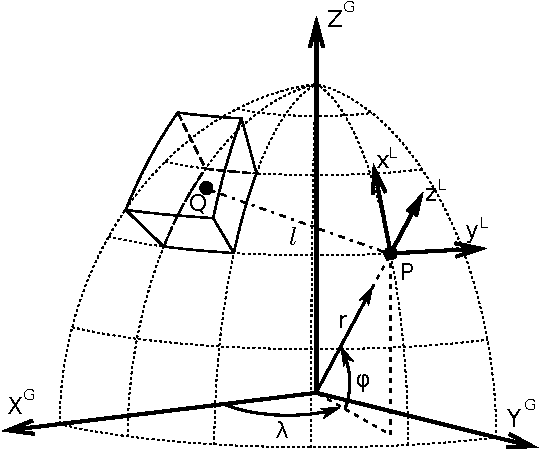
\includegraphics[scale=1]{../images/tesseroid_coordsys_other.pdf}
  \caption{\small Tesser�ide no sistema global (G) e o sistema local (L) do ponto P.
  $l$ � a dist�ncia entre o ponto P e o ponto Q pertencente ao tesser�ide.}
  \label{tess-coord-sys}
\end{figure}

\begin{figure}[!htb]
  \centering
    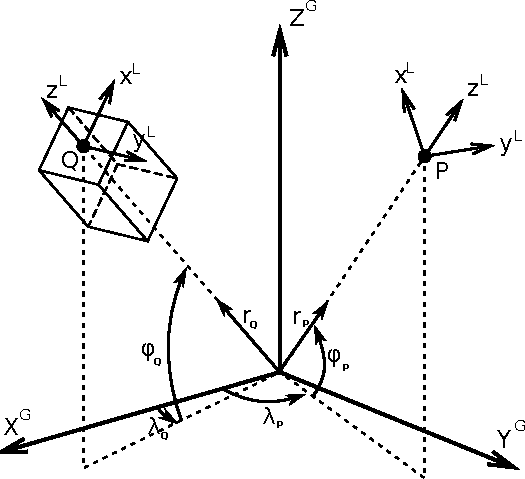
\includegraphics[scale=1]{../images/coordinate_sys.pdf}
  \caption{\small Sistemas locais dos pontos P e Q e um prisma retangular com face
           superior centrada em Q. O sistema local do ponto Q � o sistema no
           qual o TGG do prisma � calculado utilizando as f�rmulas de
           Nagy \textit{et al.} (2000). A transforma��o do TGG para o sistema
           local do ponto de observa��o P � necess�ria para dar significado
           f�sico aos resultados.}
  \label{coord-sys}
\end{figure}

  % Implementao
  \chapter{Implementa��o Computacional}

Este cap�tulo relata os aspectos computacionais e metodol�gicos do trabalho
realizado.
� discutida aqui a escolha da linguagem de programa��o para o projeto, os
algoritmos implementados e os testes de valida��o do programa desenvolvido.


\section{Linguagem de Programa��o}

O programa desenvolvido neste projeto foi implementado na linguagem Python.
A escolha desta linguagem foi baseada nas diversas vantagens que a mesma possui
sobre a linguagem C.
A principal destas � que o desenvolvimento de um programa em Python �
muito mais r�pido que o de um em C.
Al�m disso, outras vantagens importantes da linguagem Python s�o:

\begin{itemize}
  \item Sua vasta biblioteca padr�o, na qual existem m�dulos para fazer o
    processamento dos argumentos de linha de comando, automatizar os testes de
    integridade das diferentes partes do programa (chamados de Unit Tests),
    lidar com o sistema de arquivos, etc;
  \item Suporte para diversos paradigmas de programa��o, como programa��o
    orientada a objetos, programa��o seq�encial e programa��o concorrente;
  \item Pode ser utilizada na forma de scrips;
  \item Programas escritos em Python podem ser importados em scripts ou outros
    programas na forma de m�dulos, o que facilita a reutiliza��o de programas;
  \item A linguagem Python � interpretada, n�o compilada como a linguagem C.
    Logo, programas escritos nela s�o independentes do sistema operacional;
\end{itemize}

\indent Por ser interpretada, a linguagem Python possui pior performance que a
linguagem C.
No entanto, esta limita��o pode ser superada pois a linguagem Python pode ser
facilmente integrada com a linguagem C.
As partes do programa que requerem maior performance (conhecidas como
bottlenecks) podem ser substitu�das por rotinas programadas em C sem perder
todos os outro benef�cios que a linguagem Python oferece.
\\
\indent O c�digo fonte do programa desenvolvido est� hospedado no servidor
gratuito do Google Code (\texttt{http://code.google.com/p/tesseroids}) como software livre segundo os termos da GNU General
Public License 3.0. 
Isso significa que o c�digo do programa pode ser livremente acessado e
modificado por qualquer pessoa, desde que esta mantenha o c�digo aberto sob a
mesma licen�a.



\section{Implementa��o Computacional da QGL}


A QGL foi implementada na forma de um m�dulo, denominado \texttt{glq.py}, que
contem duas classes: \texttt{Abscissas} e \texttt{Weights}.
Estas classes s�o as respons�veis por calcular e armazenar os pontos de
discretiza��o e os pesos utilizados na QGL.
\\
\indent A classe \texttt{Abscissas} contem um m�todo para calcular os pontos de
discretiza��o (n�s) da QGL e outro para convert�-los para o intervalo $[a, b]$,
definido pelos limites de integra��o.
Como dito no Cap�tulo 2, os pontos de discretiza��o s�o dados pelas ra�zes
$\xi_k$ de um polin�mio de Legendre.
Para calcular essas ra�zes foi implementado um m�todo de Newton modificado para
ter uma converg�ncia maior (BARRERA-FIGUEROA \textit{et al.}, 2006).
Segundo este m�todo $k$-�sima raiz do polin�mio de Legendre $P_N(\xi)$ de ordem
$N$ pode ser calculada atrav�s de um processo iterativo:

\begin{equation}
  \xi_{k, n+1} = \xi_{k,n} -
    \dfrac{P_N(\xi_{k,n})}{P_N'(\xi_{k,n}) - P_N(\xi_{k,n})
    \displaystyle\sum\limits_{i=1}^{k-1} \dfrac{1}{\xi_{k,n} - \xi_i}}
\label{k-esima-raiz}
\end{equation}

\noindent onde os $\xi_i$ s�o as $k-1$ ra�zes que j� foram calculadas.
Esse processo � terminado quando
$\varepsilon = |\xi_{k,n+1} - \xi_{k,n}| \leqslant 10^{-15}$ ou quando um
n�mero m�ximo de $10^4$ itera��es for alcan�ado.
Os chutes iniciais para o processo iterativo foram calculados segundo
Press \textit{et al.} (1992):

\begin{equation}
  \xi_{k,0} = \dfrac{\cos\left(\pi k - \frac{\pi}{4}\right)}{N+\frac{1}{2}}
\label{chute-inicial}
\end{equation}

Como as ra�zes dos polin�mios de Legendre est�o contidas no intervalo $[-1, 1]$,
elas devem ser convertidas para o intervalo de integra��o $[a, b]$ antes de serem
utilizadas.
Esta convers�o foi feita utilizando a seguinte equa��o:

\begin{equation}
  x_k  = \dfrac{(b-a)}{2} \xi_k + \dfrac{(a+b)}{2}
\label{scale-factor}
\end{equation}

A classe \texttt{Weights} calcula os pesos associados a uma determinada inst�ncia
da classe \texttt{Abs\-cis\-sas} utilizando as equa��es \eqref{pesos} a
\eqref{rel-recur2}.




\section{C�lculo do TGG de Tesser�ides}


As classes encarregadas de calcular as seis componentes do TGG est�o contidas no
m�dulo \texttt{tesseroidgravity.py}.
Este m�dulo cont�m sete classes, sendo a principal delas a classe
\texttt{Tesseroid\-Gravity}.
Esta classe cont�m o m�todo \texttt{calculate} que utiliza a QGL para integrar uma fun��o
virtual \texttt{kernel}, cuja implementa��o � feita nas classes
\texttt{Tesseroid\-Gxx}, \texttt{Tesseroid\-Gxy}, \texttt{Tesseroid\-Gxz},
\texttt{Tesseroid\-Gyy}, \texttt{Tesseroid\-Gyz} e \texttt{Tesseroid\-Gzz} que s�o
subclasses de \texttt{Tesseroid\-Gravity}.
A fun��o \texttt{kernel} de cada subclasse corresponde ao integrando da respectiva
componente do TGG.
Assim, cada subclasse utiliza o mesmo m�todo de \texttt{Tesseroid\-Gravity} para
calcular uma componente do TGG para todos os pontos de uma grade e para todos os
tesser�ides de um modelo de entrada.
Nos c�lculos foram utilizados os valores de constante gravitacional
$G = 6,673 \times 10^{-11}\ m^3kg^{-1}s^{-2}$ e raio da Terra esf�rica
$R = 6\ 378\ 137\ m$ (WILD-PFEIFFER, 2008).
Como todos os c�lculos s�o efetuados em unidades do S.I., o resultado deve ser
convertido para E\"otvos, que � a unidade mais usual.
O fator de convers�o � $1\ \text{s}^{-2} = 10^9\ \text{E\"otvos}$.
\\
\indent O m�todo \texttt{calculate} de \texttt{Tesseroid\-Gravity} utiliza a integra��o
anal�tica na dire��o radial e integra��o num�rica da integral dupla resultante
(WILD-PFEIFFER, 2008).
Esta metodologia apresenta melhor performance que o c�lculo do TGG utilizando
somente integra��o num�rica com a QGL 3D.
Por�m, as integrais duplas apresentam uma singularidade quando o �ngulo
$\psi$ entre o ponto de observa��o e o ponto de integra��o � igual a zero.
Essa singularidade n�o est� presente nas integrais triplas.
\\
\indent No contexto da QGL a singularidade ocorre se o ponto de observa��o
possuir mesma latitude e longitude que um dos pontos de discretiza��o (n�s).
Computacionalmente, essa singularidade provoca um ``erro de divis�o por zero''
que termina o programa.
Para contornar este problema, nos pontos de observa��o onde este erro ocorre o
TGG passa a ser calculado utilizando a QGL 3D, evitando a singularidade.



\section{C�lculo do TGG de Prismas Retangulares}

O c�lculo do TGG utilizando a distribui��o de massa em prismas retangulares foi
implementada para estimar o erro da aproxima��o plana para a Terra esf�rica.
Para isso, cada tesser�ide foi aproximado por um prisma retangular com o mesmo
volume, densidade e altura do tesser�ide.
Assumindo que o tesser�ide � muito pequeno quando comparado � Terra
($\sin\Delta\varphi = \Delta\varphi$) e que sua altura � muito menor que sua
dist�ncia at� a origem do sistema global ($\Delta r \ll r_1$), as dimens�es do
prisma retangular s�o dadas por (WILD-PFEIFFER, 2008):


\begin{subequations}
\begin{align}
  \Delta x &= \dfrac{r_1 + r_2}{2} \Delta \varphi
  \label{tess2prism-dx}
\\[4mm]
  \Delta y &= \dfrac{r_1 + r_2}{2} \cos \left(\dfrac{\varphi_1 + \varphi_2}{2}
    \right) \Delta \lambda
  \label{tess2prism-dy}
\\[4mm]
  \Delta z &= \Delta r
  \label{tess2prism-dz}
\end{align}
\end{subequations}

\indent As f�rmulas anal�ticas de $V$ e suas derivadas para um prisma retangular
de densidade constante $\rho$ s�o dadas em Nagy \textit{et al.} (2000).
Nesta formula��o foi assumida uma aproxima��o plana para a Terra.
Conseq�entemente o sistema local do prisma tem a mesma orienta��o do sistema
local do ponto de observa��o.
Por�m, se o prisma retangular, ou um conjunto deles, for utilizado para
representar um segmento esf�rico da Terra, o sistema local do ponto de
observa��o n�o ter� a mesma orienta��o do sistema local do prisma
(Figura \ref{coord-sys}).
Logo, neste caso � necess�rio converter o TGG para o sistema local do ponto de
observa��o utilizando a matriz de transforma��o apresentada na equa��o
\eqref{tranf-QtoP}.

\begin{equation}
  T^{L_{ob}} = R\ T^{L_{pr}} R^T
\label{tgg-transf}
\end{equation}

\noindent onde $T^{L_{ob}}$ � o TGG no sistema local do ponto de observa��o e
$T^{L_{pr}}$ � o TGG no sistema local do prisma.
\\
\indent Para utilizar as f�rmulas de Nagy \textit{et al.} (2000) � necess�rio
conhecer tamb�m as coordenadas do ponto de observa��o no sistema local do prisma
(Figura \ref{coord-sys}).
Este sistema difere do sistema utilizado em Nagy \textit{et al.} (2000) somente
no sentido da componente $z$ (Figura \ref{nagy-cood-sys}).
Assim, a transforma��o das coordenadas do ponto de observa��o do sistema global
para o sistema local do prisma pode ser feita utilizando a equa��o
\eqref{tranf-GtoP} e invertendo o sinal da componente $z$.
Nessa equa��o, $\mathbf{e}^{L_P}_Q$ passa a representar o vetor posi��o do ponto
de observa��o no sistema local do prisma, $\mathbf{e}^{G}_Q$ o vetor posi��o do
ponto de observa��o no sistema global e $\mathbf{e}^{G}_Q$ o vetor posi��o da
origem do sistema local do prisma no sistema global.
Por conven��o, a origem do sistema local do prisma est� localizada no centro de
sua face superior.




\section{C�lculo do TGG de uma Casca Esf�rica}


Para validar os resultados obtidos com o programa computacional implementado, �
necess�rio compar�-los com valores obtidos atrav�s de f�rmulas anal�ticas.
Um modelo 3D para o qual existe uma f�rmula anal�tica � uma casca esf�rica com
densidade e espessura constantes (Figura \ref{sph-cap}).
O potencial desta casca esf�rica � dado por:

\begin{equation}
  V \left(r, \varphi, \lambda \right) = G \rho
    \int\limits_{r_1}^{r_2}
    \int\limits_{\varphi_c}^{\frac{\pi}{2}}
    \int\limits_{0}^{{2\pi}}
    \dfrac{1}{l}\ r'^2 \cos\varphi'\ d\lambda'\ d\varphi'\ d r'
\label{sphcap-pot}
\end{equation}

\indent Se o ponto de observa��o estiver localizado ao longo do eixo $Z$ do
sistema global, a equa��o \eqref{sphcap-pot} resulta em (HECK; SEITZ, 2007):

\begin{multline}
 V \left(r, \varphi=\frac{\pi}{2}, \lambda=0 \right) = 2 \pi G \rho
  \Biggl\{
    \dfrac{l_c^3}{3r}
    + \dfrac{r^2 \sin\varphi_c \cos^2\varphi_c}{2}\ln(l_c + r' - r \sin\varphi_c)
    \\    
    + \dfrac{r'^3}{3r} - \dfrac{r'^2}{2} 
     + \dfrac{l_c \sin \varphi_c}{2} (r' - r \sin \varphi_c)
  \Biggr\} \Biggr\rvert^{r'=r_2}_{r'=r_1}
\label{sphcap-pot-polo}
\end{multline}

\noindent onde

\[
  l_c = \sqrt{r'^2 + r^2 - 2rr'\sin\varphi_c}
\]

\indent A partir da equa��o \eqref{sphcap-pot-polo} � poss�vel obter o TGG
causado pela casca esf�rica.
Devido � simetria do modelo e � localiza��o do ponto de observa��o,
as equa��es \eqref{txx-esf} a \eqref{tzz-esf} podem ser simplificadas para
(WILD-PFEIFFER, 2008):

\begin{subequations}
\begin{align}
  T_{xx} &= T_{yy} = - \dfrac{1}{2} \dfrac{\partial^2 V}{\partial r^2}
  \label{sphcap-txx-tyy}
  \\
  T_{xy} &= T_{yx} = 0
  \label{sphcap-txy}
  \\
  T_{xz} &= T_{zx} = 0
  \label{sphcap-txz}
  \\
  T_{yz} &= T_{zy} = 0
  \label{sphcap-tyz}
  \\
  T_{zz} &= \dfrac{\partial^2 V}{\partial r^2}
  \label{sphcap-tzz}
\end{align}
\end{subequations}

\noindent onde a segunda derivada de $V$ na dire��o radial � dada por:

\begin{multline}
  \dfrac{\partial^2 V}{\partial r^2} = 2 \pi G \rho \Biggl\{
    \dfrac{2 l_c^3}{3 r^3}
    - \dfrac{l_c}{r^2}(r - 2r' \sin\varphi_c)
    + \dfrac{r - r' \sin\varphi_c}{l_c}
    - \dfrac{r' \sin\varphi_c}{r l_c}(r - r'\sin\varphi_c)
  \\[4mm]
    - \dfrac{\sin^2\varphi_c}{2l_c}(r - r'\sin\varphi_c)
    + \dfrac{2 r'^3}{3 r^3}
  \\[4mm]
    + \dfrac{\sin\varphi_c}{2} \left[
      \dfrac{r' - 2r\sin\varphi_c + r' \sin^2\varphi_c}{l_c}
      - \dfrac{(r - r'\sin\varphi_c)^2(r' - r\sin\varphi_c)}{l_c^3}
    \right]
  \\[4mm]
    + \sin\varphi_c \cos^2\varphi_c \left[
      \ln(l_c + r' - r \sin\varphi_c) + \dfrac{r}{l_c + r' - r \sin\varphi_c}
      \left( \dfrac{r - r'\sin\varphi_c}{l_c} - \sin\varphi_c \right)
    \right]
  \\[4mm]
    + \dfrac{\sin\varphi_c \cos^2\varphi_c}{2 l_c (l_c + r' - r \sin\varphi_c)}
    \left[
      3r^2 - 2 r l_c \sin\varphi_c -
      \dfrac{r^2}{l_c}\sin\varphi_c(r - r'\sin\varphi_c) -
      2r r' \sin\varphi_c
    \right]
  \\[4mm]
    - \dfrac{\sin\varphi_c \cos^2\varphi_c r^2( r- (l_c + r') \sin\varphi_c)}
    {2 l_c^2 (l_c + r' - r \sin\varphi_c)^2}  \Biggl[
      2(r - r'\sin\varphi_c)
  \\[4mm]
      + \dfrac{r'}{l_c}(r - r'\sin\varphi_c)
      - l_c \sin\varphi_c
      - \dfrac{r \sin\varphi_c}{l_c}(r - r'\sin\varphi_c) \Biggr]
    \Biggr\}
    \Biggr\rvert^{r'=r_2}_{r'=r_1}
\label{sphcap-seg-deriv}
\end{multline}

\indent A equa��o \eqref{sphcap-seg-deriv} pode ser utilizada para calcular o
TGG causado por um anel de massa com $\Delta\varphi = \varphi_{i+1} - \varphi_i$
subtraindo o efeito de duas cascas esf�ricas de raio esf�rico
$\varphi_c = \varphi_{i+1}$ e $\varphi_c = \varphi_{i}$ (Figura \ref{sph-cap}).
Assim � poss�vel analisar como a dist�ncia entre o modelo e o ponto de
observa��o afeta o erro do programa computacional desenvolvido.



% FIGURAS
\newpage
\begin{figure}[!htb]
  \centering
    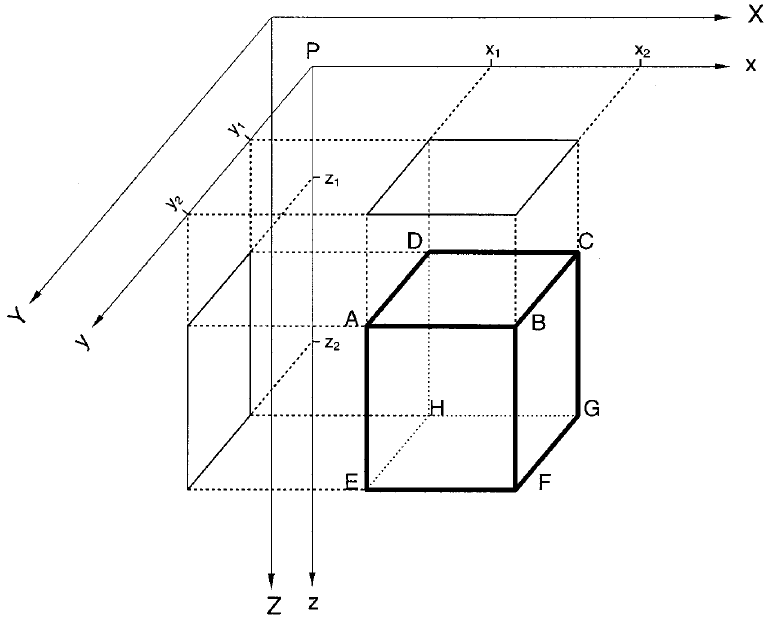
\includegraphics[scale=0.35]{../images/prism_coord_sys.png}
  \caption{\small Sistemas de coordenadas utilizados em Nagy \textit{et al.} (2000).
    O sistema (x,y,z) com origem no ponto de observa��o P � o utilizado na
    formula��o. Para realizar os c�lculos, � necess�rio conhecer as coordenadas
    do ponto P no sistema local do prisma ABCDEFGH.
    Fonte Nagy \textit{et al.} (2000)}
  \label{nagy-cood-sys}
\end{figure}

\begin{figure}[!htb]
  \centering
    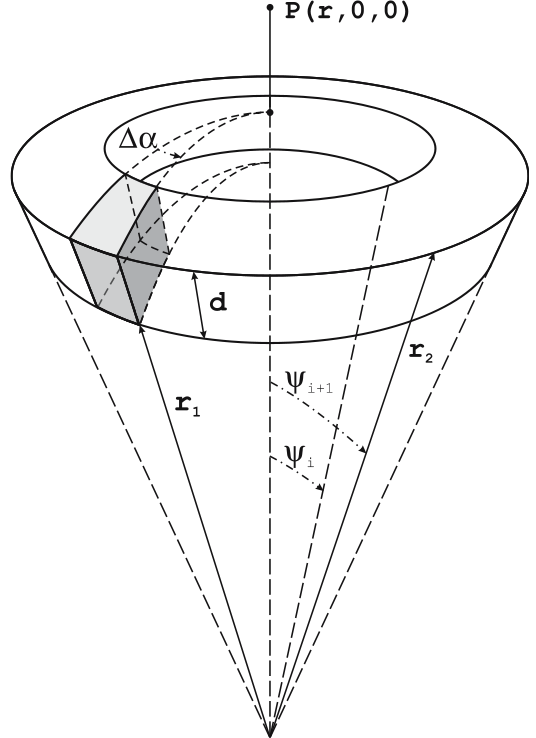
\includegraphics[scale=0.35]{../images/spherical_shell.png}
  \caption{\small Anel de massa obtido subtraindo as cascas esf�ricas de raio esf�rico
    $\psi_{i+1}$ e $\psi_i$ ($\psi = 90^\circ - \varphi_c$). O ponto de
    observa��o P est� localizado ao longo do eixo $Z$ global.
    Fonte Heck e Seitz (2007).}
  \label{sph-cap}
\end{figure}


  % Resultados
  \chapter{Resultados}



\section{Valida��o do programa desenvolvido}

Com o objetivo de testar se o programa computacional desenvolvido est�
funcionando corretamente, foi feita a compara��o entre os resultados previstos
analiticamente por um anel de massa (Wild-Pfeiffer, 2008) com aqueles previstos
pela aproxima��o por tesser�ides.
\\
\indent A Figura \ref{sphcap-tgg-diag} apresenta as componentes n�o nulas do TGG causado
por an�is de massa de $\Delta \varphi = 5'$, $\rho = 2\ 670\ kg\ m^{-3}$,
$\Delta r = 1\ 000\ m$ e ponto de observa��o no p�lo Norte a 250 km de altitude.
Para comparar estes resultados com o do programa desenvolvido, cada anel foi
discretizado em tesser�ides de  $5' \times 5' \times 1\ km$ e foram utilizadas
ordens de QGL ($N_\varphi = N_\lambda$) dois, tr�s, quatro e cinco, segundo
Wild-Pfeiffer (2008).
As diferen�as entre os dois resultados est�o apresentados na Figura
\ref{sphcap-tgg-dif} e nas Tabelas \ref{tabela-diff-cap-tess-diag} e
\ref{tabela-diff-cap-tess-nondiag}.
\\
\indent As componentes $T_{xx}$ e $T_{zz}$ apresentam diferen�as de aproxima��o
m�ximas da ordem de $10^{-9}$ e $10^{-8}$ E\"otvos, respectivamente, para
$N_\varphi = N_\lambda = 2$.
Essas diferen�as s�o $10^7$ vezes menores do que os valores previstos
pelas formulas anal�ticas.
Para $N_\varphi = N_\lambda > 2$, as diferen�as m�ximas diminuem para $10^{-12}$
E\"otvos.
Para an�is abaixo de $\varphi_c = 85^\circ$ a ordem da QGL deixa de influenciar
significantemente a diferen�a.
J� as componentes $T_{xz}$ e $T_{yz}$ apresentam diferen�as m�ximas da ordem de
$10^{-15}$ E\"otvos, independente de $N_\varphi$ e $N_\lambda$.
Nestas componentes a diferen�a estabiliza para $\varphi_c < 85^\circ$.
\\
\indent As componentes $T_{xy}$ e $T_{yy}$ apresentam diferen�as m�ximas da
ordem de $10^{-3}$ E\"otvos, para todos os valores de $N_\varphi$ e $N_\lambda$
utilizados.
Essas componentes apresentam comportamento crescentemente inst�vel com a
varia��o de $\varphi_c$, independente da ordem da QGL.
Esta instabilidade era esperada pois quando $\varphi = \pm 90^\circ$ o termo
$\cos^{-2}\varphi$ das equa��es \eqref{txy-esf} e \eqref{tyy-esf} �
numericamente inst�vel.
Idealmente, $\cos(\pm90^\circ)=0$ e geraria um erro computacional de ``divis�o por
zero'' que terminaria o programa.
Por�m, o cosseno � aproximado por uma s�rie e
$\cos^{-2}(\pm90^\circ)\approx10^{32}$, gerando os valores altos nas diferen�as
observadas na Figura \ref{sphcap-tgg-dif}.
Este mesmo efeito n�o � observado na componente $T_{yz}$ (equa��o
\eqref{tyz-esf}) pois o termo $\cos^{-1}\varphi$ � cancelado quando multiplicado
pelo termo $\cos\varphi$ presente em $\frac{\partial^2 V}{\partial r \partial\lambda}$ e
$\frac{\partial V}{\partial\lambda}$.



\section{Exemplo do TGG causado por um tesser�ide}
    
O programa desenvolvido foi utilizado para calcular o TGG causado por um
tesser�ide de $1^\circ \times 1^\circ \times 10\ km$,
$\rho = 2\ 800\ kg\ m^{-3}$, centrado em $40^\circ \text{N}$ e
$83^\circ \text{W}$ e observado a 250 km de altitude, como em  Asgharzadeh
\textit{et al.} (2007).
A ordem de QGL utilizada foi $N_\varphi = N_\lambda = 2$, enquanto em
Asgharzadeh \textit{et al.} (2007) foi utilizada QGL 3D com ordem
$N_\varphi = N_\lambda = 8$ e $N_r = 2$.
O resultado deste c�lculo est� apresentado na Figura \ref{vonfrese-tgg} e �
semelhante ao apresentado em Asgharzadeh \textit{et al.} (2007) tanto em forma
como em magnitude.
Isto serve para validar resultado do programa desenvolvido em um caso
diferente do dos an�is de massa com ponto de observa��o localizado no p�lo.



\section{Limita��es Num�ricas}

Ku (1977) observou que se a dist�ncia entre os n�s da QGL for maior que a
dist�ncia ao ponto de observa��o, o TGG aparenta ser causado por massas pontuais
localizadas nos n�s.
Este � um artefato num�rico da QGL que foi observado para o caso da componente
vertical da acelera��o da gravidade.
Para que esse artefato n�o ocorra, Ku (1977) prop�s aumentar o n�mero de n�s at�
que a dist�ncia entre os mesmos fosse menor que a dist�ncia at� o ponto de
observa��o.
\\
\indent Para verificar se o artefato observado por Ku (1977) tamb�m ocorre com o
TGG, o mesmo foi calculado para um tesser�ide de
$2^\circ \times 2^\circ \times 10\ km$ e densidade $\rho = 2\ 800\ kg\ m^{-3}$ a
diversas altitudes.
A Figura \ref{tgg-ku-250} mostra o TGG calculado a 250 km de altitude utilizando
$N_\varphi = N_\lambda = 2$.
Neste caso, a dist�ncia entre dois n�s adjacentes � de aproximadamente 128,5 km.
Nota-se que o TGG possui forma semelhante ao apresentado na Figura
\ref{vonfrese-tgg}.
No entanto, quando o c�lculo � efetuado a 100 km de altitude, a componente
$T_{zz}$ aparenta ser causada por massas pontuais localizadas nos n�s (Figura
\ref{tgg-ku-100}).
Esse efeito pode ser claramente observado em todas as componentes quando o TGG �
calculado a 50 km de altitude (Figura \ref{tgg-ku-50-o2}).
\\
\indent Se o n�mero de n�s for aumentando para $N_\varphi = N_\lambda = 10$,
a dist�ncia entre dois n�s adjacentes diminui para aproximadamente 33 km.
Pode ser notado na Figura \ref{tgg-ku-50-o10} que o TGG calculado a 50 km de
altitude com esse n�mero de n�s n�o apresenta ser causado por massas pontuais.
De fato, o mesmo se assemelha ao TGG causado por um prisma que aproxima o
tesser�ide como descrito na Se��o 3.4 (Figura \ref{tgg-ku-50-prisma}).



\section{Analise num�rica  da aproxima��o plana sobre o TGG}

A aproxima��o plana para a Terra esf�rica geralmente consiste em aproximar um corpo curvo
por um corpo plano e efetuar a computa��o em uma grade tamb�m plana.
Isto significa assumir que os sistemas locais dos pontos de observa��o possuem a
mesma orienta��o do sistema local do corpo plano e que $1^\circ$ de latitude ou
longitude equivale a 111,11 km.
A diferen�a causada no TGG por essa aproxima��o foi quantificada subtraindo o
TGG causado por um tesser�ide do causado por um prisma retangular de mesma massa,
calculado utilizando a aproxima��o descrita acima.
\\
\indent A diferen�a calculada para um tesser�ide de
$1^\circ \times 1^\circ \times 10\ km$ e $\rho = 2\ 800\ kg\ m^{-3}$ est�
apresentada na Figura \ref{tgg-dif1x1}.
As diferen�as chegam a aproximadamente 7\% na componente $T_{xy}$, por�m n�o
passam de 0.5\% na componente $T_{zz}$.
Estas diferen�as s�o m�nimas e geralmente s�o ignoradas na modelagem de estruturas
pequenas.
Por�m, quando o modelo � um tesser�ide de
$50^\circ \times 50^\circ \times 10\ km$, as diferen�as chegam a aproximadamente
30\% na componente $T_{zz}$ e aproximadamente 5\% na componente $T_{xy}$
(Figura \ref{tgg-dif50x50}).
Esta � uma diferen�a significativa e deve ser levada em conta na modelagem de
estruturas extensas.




\section{Efeito topogr�fico}

Os dados de TGG que ser�o obtidos pelo sat�lite GOCE incluir�o o efeito
gravitacional da topografia.
Neste trabalho foi feita uma primeira estimativa da amplitude deste efeito sobre
o TGG utilizando o programa computacional desenvolvido.
\\
\indent O efeito que as massas topogr�ficas da regi�o da bacia do Paran� exercem
sobre as componentes do TGG foi calculado utilizando o
modelo digital ETOPO1 (AMANTE; EAKINS, 2009).
Para isso, foi gerado um modelo de tesser�ides a partir de uma grade de
topografia de $10' \times 10'$ (Figura \ref{topografia}).
A densidade utilizada foi de $2\ 670\ kg\ m^{-3}$ e a ordem da QGL
$N_\varphi = N_\lambda = 2$.
O TGG foi calculado na regi�o marcada pelo ret�ngulo vermelho na Figura
\ref{topografia} e o resultado est� apresentado na Figura \ref{tgg-topografia}.
Observa-se que as amplitudes das componentes do TGG calculado possuem a mesma
ordem de grandeza das amplitudes das componentes do TGG gerado pelo tesser�ide
mostrado na Figura \ref{vonfrese-tgg}.
Este tesser�ide poderia representar uma anomalia de densidade situada na crosta
superior.
Logo, o efeito topogr�fico deve ser removido do TGG total medido com a
finalidade de isolar o efeito gravitacional causado por anomalias de densidade
situadas na parte mais interna da Terra.




% FIGURAS E TABELAS
\newpage
\begin{table}[!htb]
    \begin{center}
    \begin{normalsize}
    \begin{tabular}{c c c c}
        \toprule
           &  \multicolumn{3}{c}{Diferen�as M�ximas [E\"otvos]}\\
        \cmidrule{2-4}
        $N_\varphi = N_\lambda$ & $T_{xx}$ & $T_{yy}$ & $T_{zz}$\\
        \midrule
        2 & $6.4624 \times 10^{-9}$ & $2.7928 \times 10^{-3}$ & $1.2925 \times 10^{-8}$\\
        3 & $4.2351 \times 10^{-12}$ & $2.2529 \times 10^{-3}$ & $9.2808 \times 10^{-12}$\\
        4 & $4.5904 \times 10^{-12}$ & $2.2541 \times 10^{-3}$ & $9.0402 \times 10^{-12}$\\
        5 & $4.5907 \times 10^{-12}$ & $2.3230 \times 10^{-3}$ & $8.8367 \times 10^{-12}$\\
        \bottomrule
    \end{tabular}
    \end{normalsize}
    \end{center}
    \caption{\small Diferen�as m�ximas nas componentes diagonais do TGG entre os
      valores previstos pela
      aproxima��o por tesser�ides (programa computacional desenvolvido) e
      valores previstos pela f�rmula anal�tica de an�is de massa de
      $\Delta \varphi = 5'$, $\rho = 2\ 670\ kg\ m^{-3}$ e
      $\Delta r = 1\ 000\ m$. Cada anel foi discretizado em tesser�ides de
      $5' \times 5' \times 1\ km$. $N_\varphi$ e $N_\lambda$ s�o a ordem da QGL
      nas dire��es latitudinal e longitudinal, respectivamente.}
    \label{tabela-diff-cap-tess-diag}
\end{table}

\begin{table}[!htb]
    \begin{center}
    \begin{normalsize}
    \begin{tabular}{c c c c}
        \toprule
           &  \multicolumn{3}{c}{Diferen�as M�ximas [E\"otvos]}\\
        \cmidrule{2-4}
        $N_\varphi = N_\lambda$ & $T_{xy}$ & $T_{xz}$ & $T_{yz}$\\
        \midrule
        2 & $1.5994 \times 10^{-3}$ & $6.0564 \times 10^{-15}$ & $2.7231 \times 10^{-15}$\\
        3 & $1.4357 \times 10^{-3}$ & $6.0744 \times 10^{-15}$ & $2.7637 \times 10^{-15}$\\
        4 & $1.0552 \times 10^{-3}$ & $5.9915 \times 10^{-15}$ & $2.7706 \times 10^{-15}$\\
        5 & $8.7854 \times 10^{-4}$ & $5.9918 \times 10^{-15}$ & $2.7366 \times 10^{-15}$\\
        \bottomrule
    \end{tabular}
    \end{normalsize}
    \end{center}
    \caption{\small Diferen�as m�ximas nas componentes n�o-diagonais do TGG
      entre os valores previstos pela
      aproxima��o por tesser�ides (programa computacional desenvolvido) e
      valores previstos pela f�rmula anal�tica de an�is de massa de
      $\Delta \varphi = 5'$, $\rho = 2\ 670\ kg\ m^{-3}$ e
      $\Delta r = 1\ 000\ m$. Cada anel foi discretizado em tesser�ides de
      $5' \times 5' \times 1\ km$. $N_\varphi$ e $N_\lambda$ s�o a ordem da QGL
      nas dire��es latitudinal e longitudinal, respectivamente.}
    \label{tabela-diff-cap-tess-nondiag}
\end{table}


\begin{figure}[!htb]
  \centering
    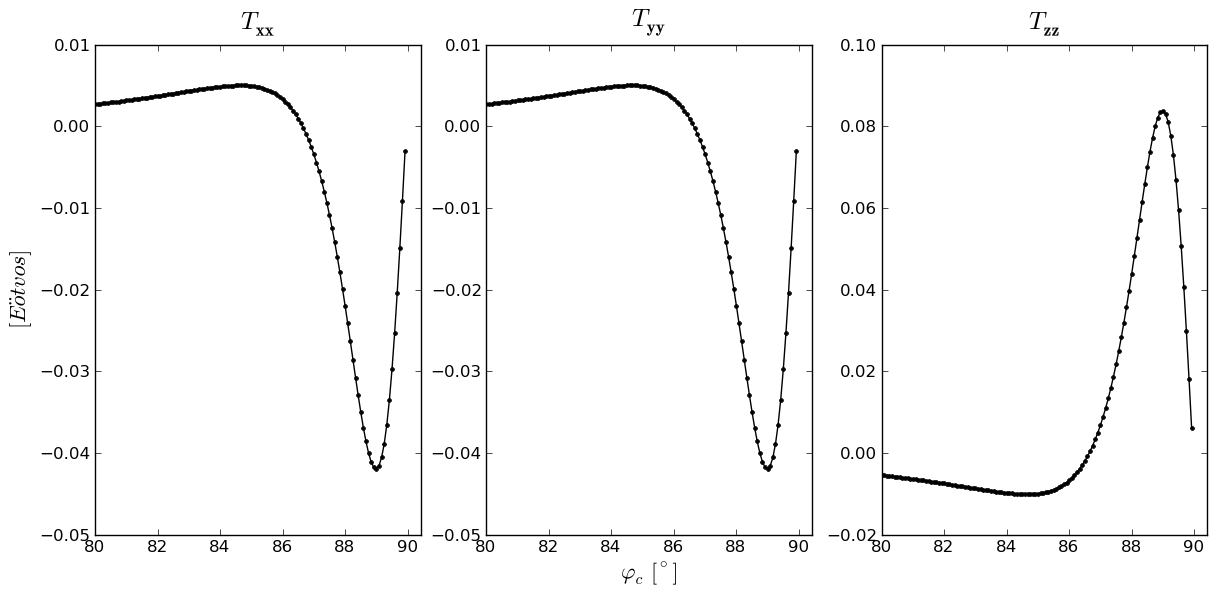
\includegraphics[scale=0.4]{../images/ggt-cap-at250.png}
  \caption{\small Componentes diagonais do TGG causado por an�is de massa de
    $\Delta\varphi = 5'$, $\rho = 2\ 670\ kg\ m^{-3}$, $\Delta r = 1\ 000\ m$
    e ponto de observa��o no p�lo Norte a $250\ km$ de altitude. $\varphi_c$ �
    a latitude do limite Sul do anel.}
  \label{sphcap-tgg-diag}
\end{figure}

\begin{figure}[!htb]
  \centering
    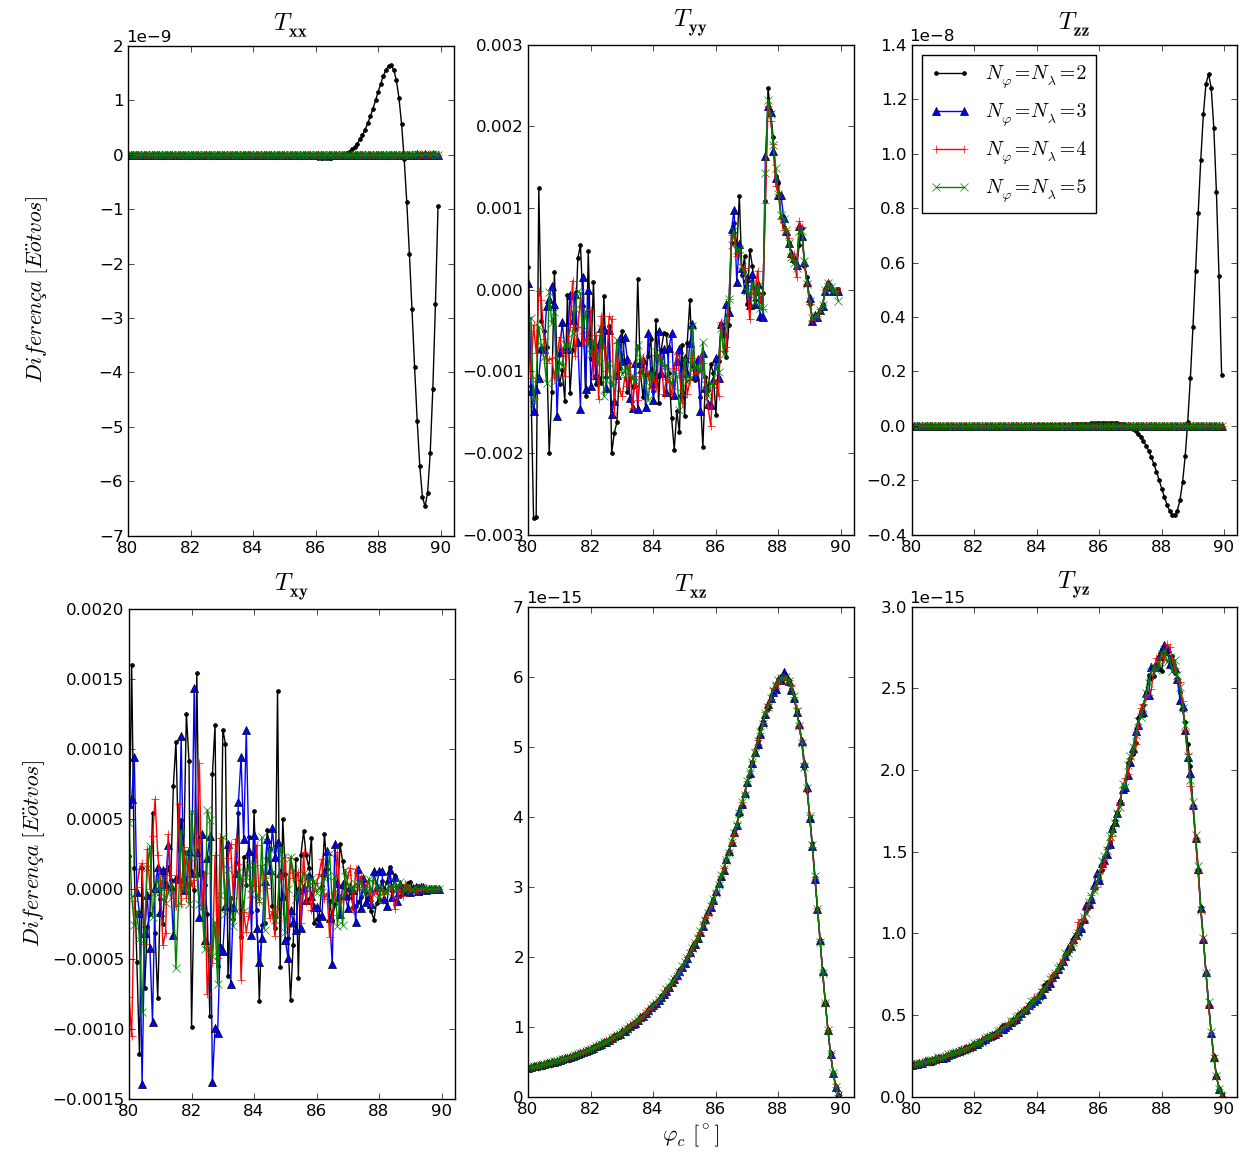
\includegraphics[scale=0.4]{../images/ggt-diffs-at250.png}
  \caption{\small Diferen�a entre o TGG calculado pelo programa desenvolvido e o
    resultado anal�tico para an�is de massa de $\Delta\varphi = 5'$,
    $\rho = 2\ 670\ kg\ m^{-3}$, $\Delta r = 1\ 000\ m$. Cada anel foi
    discretizado em tesser�ides de $5'\times5'\times1000\ m$. $N_\varphi$ e
    $N_\lambda$ s�o a ordem da QGL nas dire��es latitudinal e longitudinal,
    respectivamente.}
  \label{sphcap-tgg-dif}
\end{figure}

\begin{figure}[!htb]
  \centering
    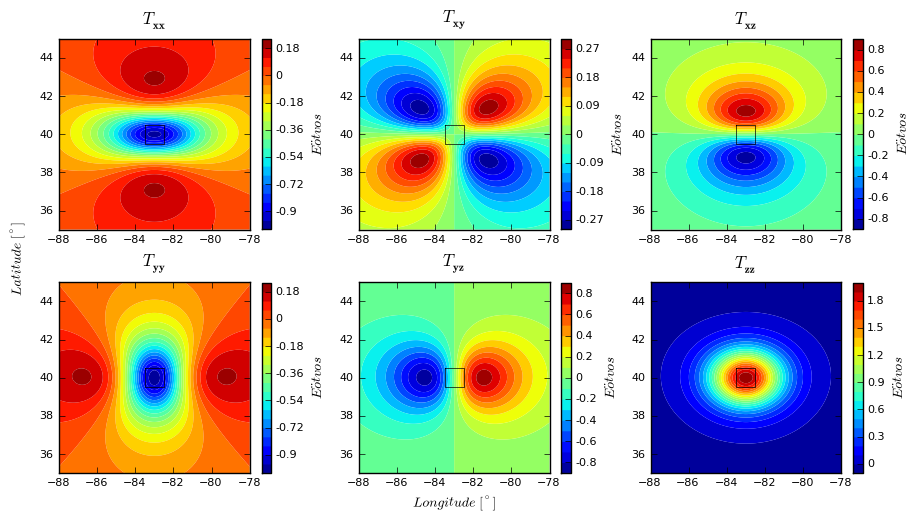
\includegraphics[scale=0.65]{../images/ggtT1x1at250-exemplo.png}
  \caption{\small TGG causado por um tesser�ide de
    $1^\circ \times 1^\circ \times 10\ km$ e densidade $2\ 800\ kg\ m^{-3}$,
    observado a $250\ km$ de altitude. O tesser�ide est� centrado em
    $40^\circ \text{N}$ e $83^\circ \text{W}$. A ordem de QGL utilizada foi
    $N_\varphi = N_\lambda = 2$. Este resultado � semelhante ao apresentado
    em Asgharzadeh \textit{et al.} (2007). As bordas do tesser�ide est�o
    marcadas em preto no centro dos mapas.}
  \label{vonfrese-tgg}
\end{figure}

\begin{figure}[!htb]
  \centering
    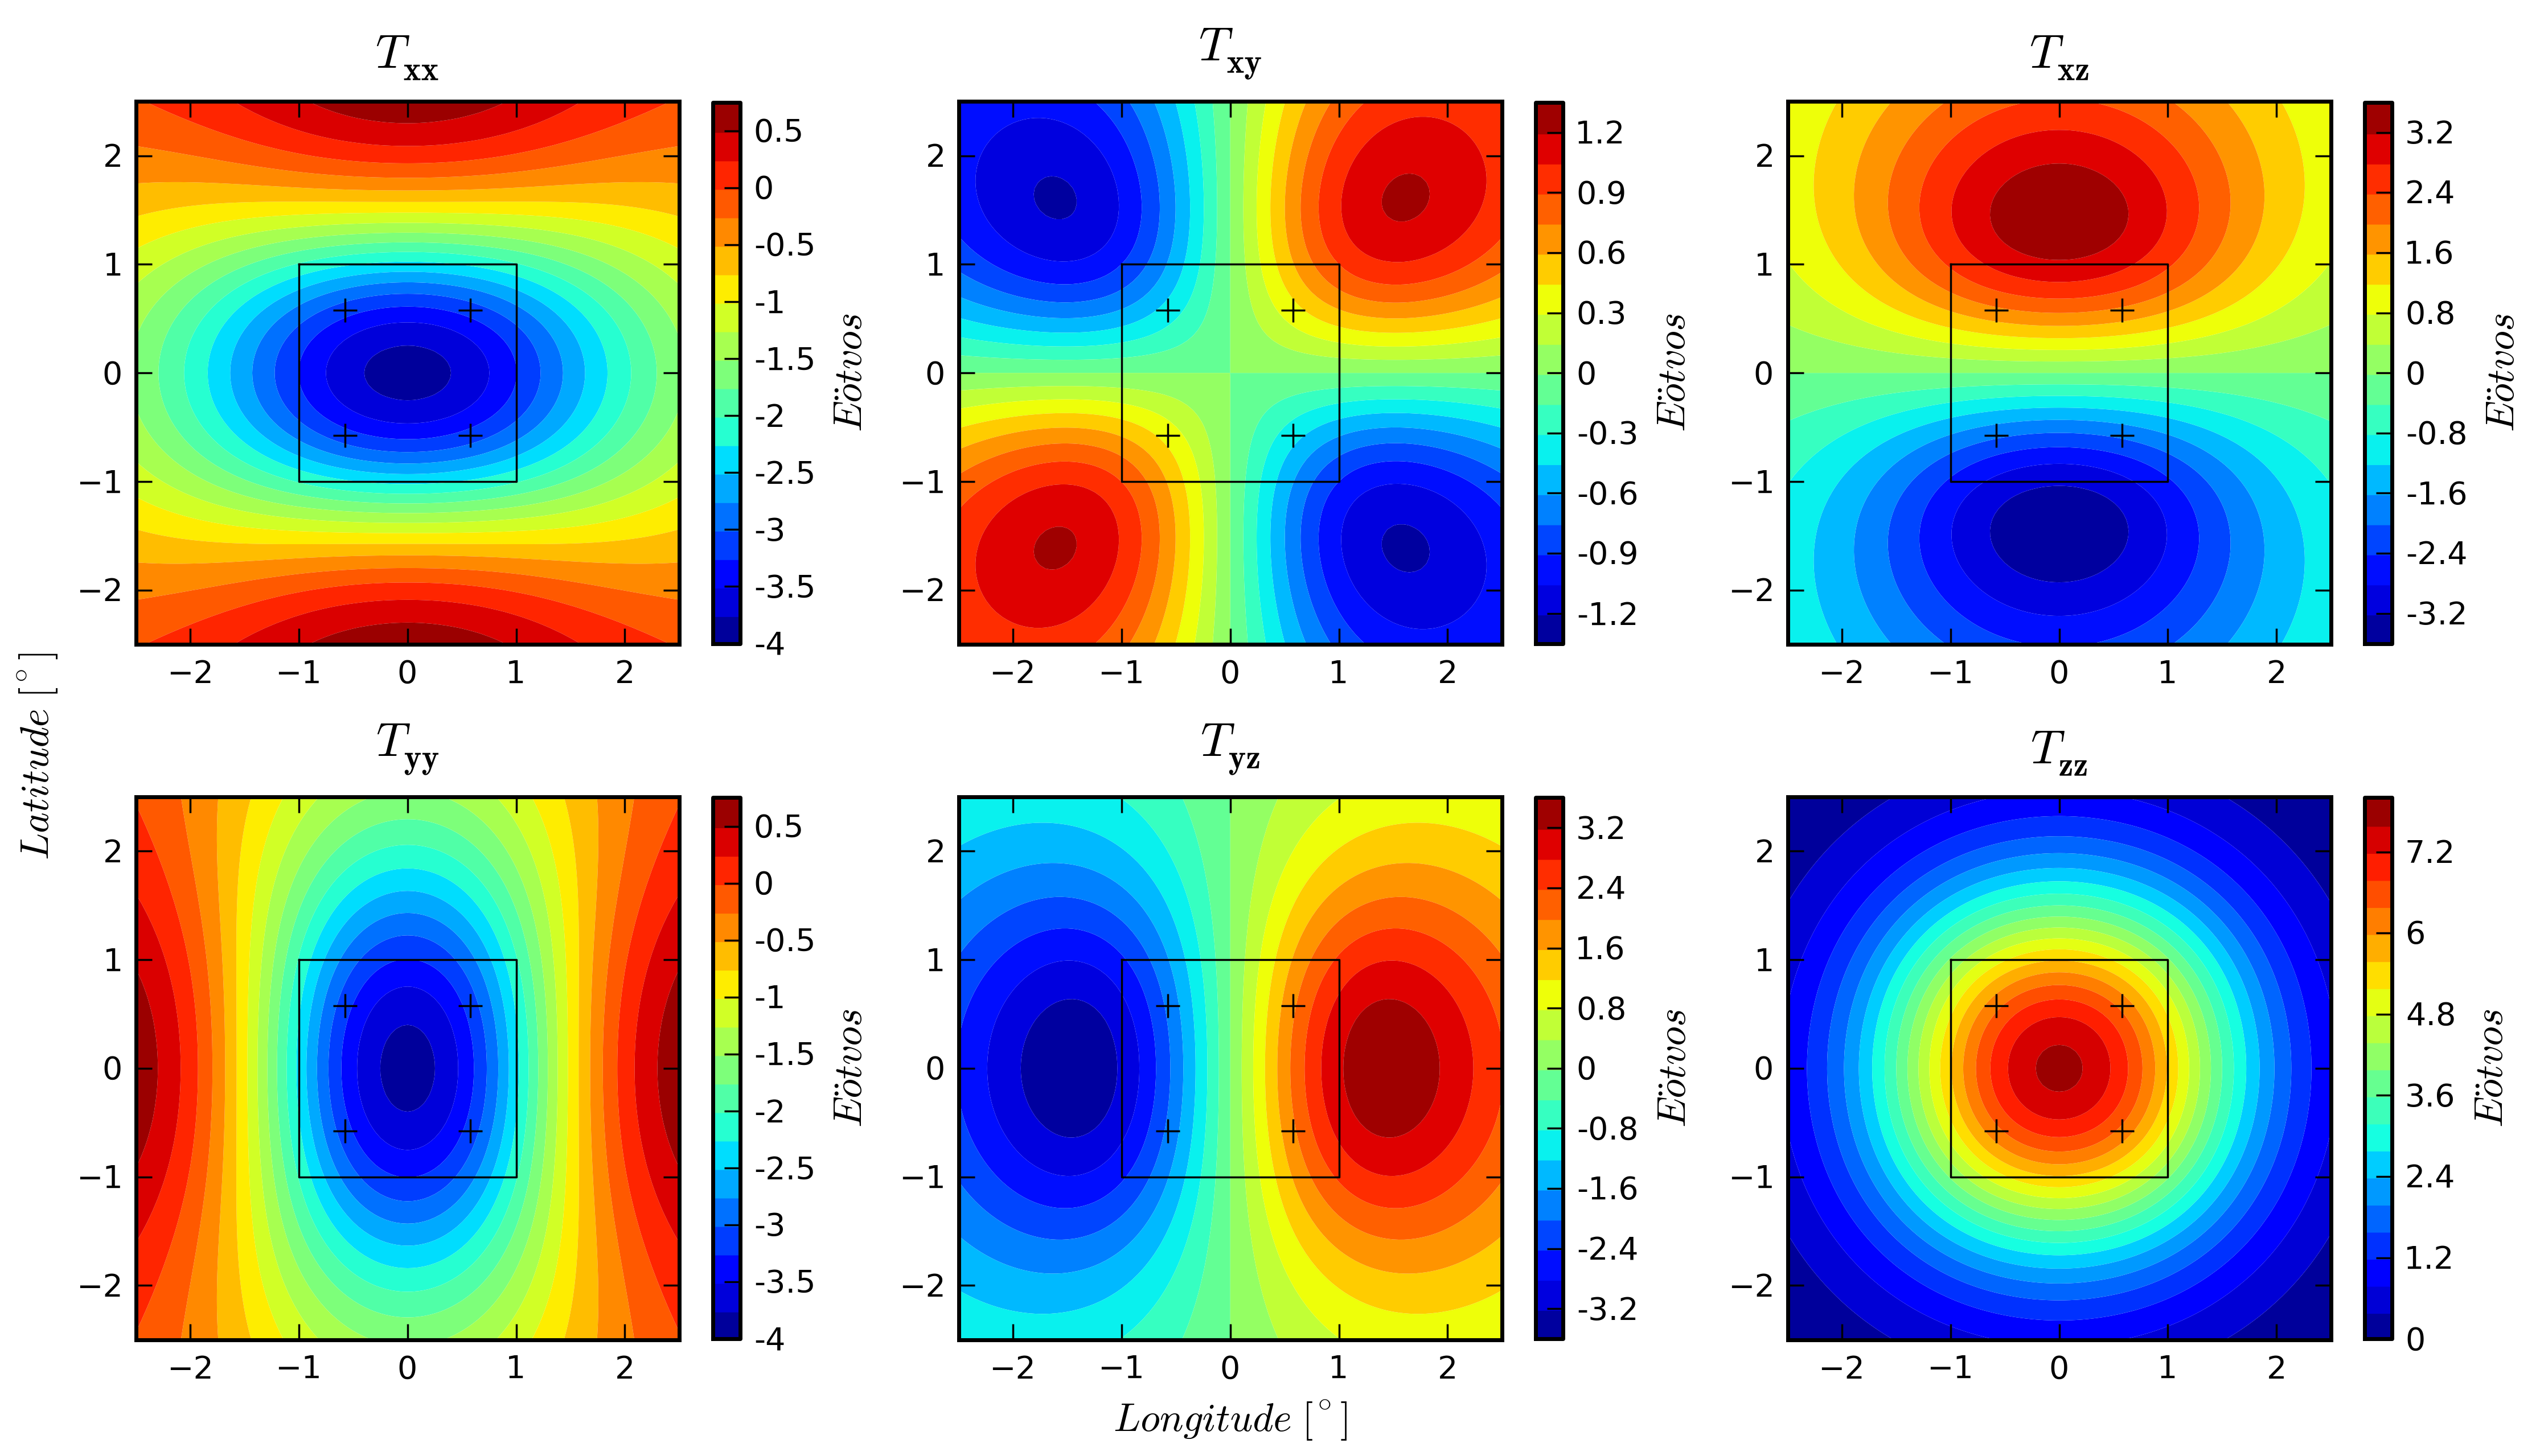
\includegraphics[scale=0.67]{../images/ku2x2at250-o2.png}
  \caption{\small TGG causado por um tesser�ide de
    $2^\circ \times 2^\circ \times 10\ km$, com densidade $2\ 800\ kg\ m^{-3}$,
    calculado a $250\ km$ de altitude. A ordem utilizada foi
    $N_\varphi = N_\lambda = 2$. As bordas do tesser�ide est�o marcadas em preto
    e os s�mbolos $+$ s�o os n�s da QGL. A dist�ncia entre dois n�s adjacentes
    � de aproximadamente $128,5\ km$.}
  \label{tgg-ku-250}
\end{figure}

\begin{figure}[!htb]
  \centering
    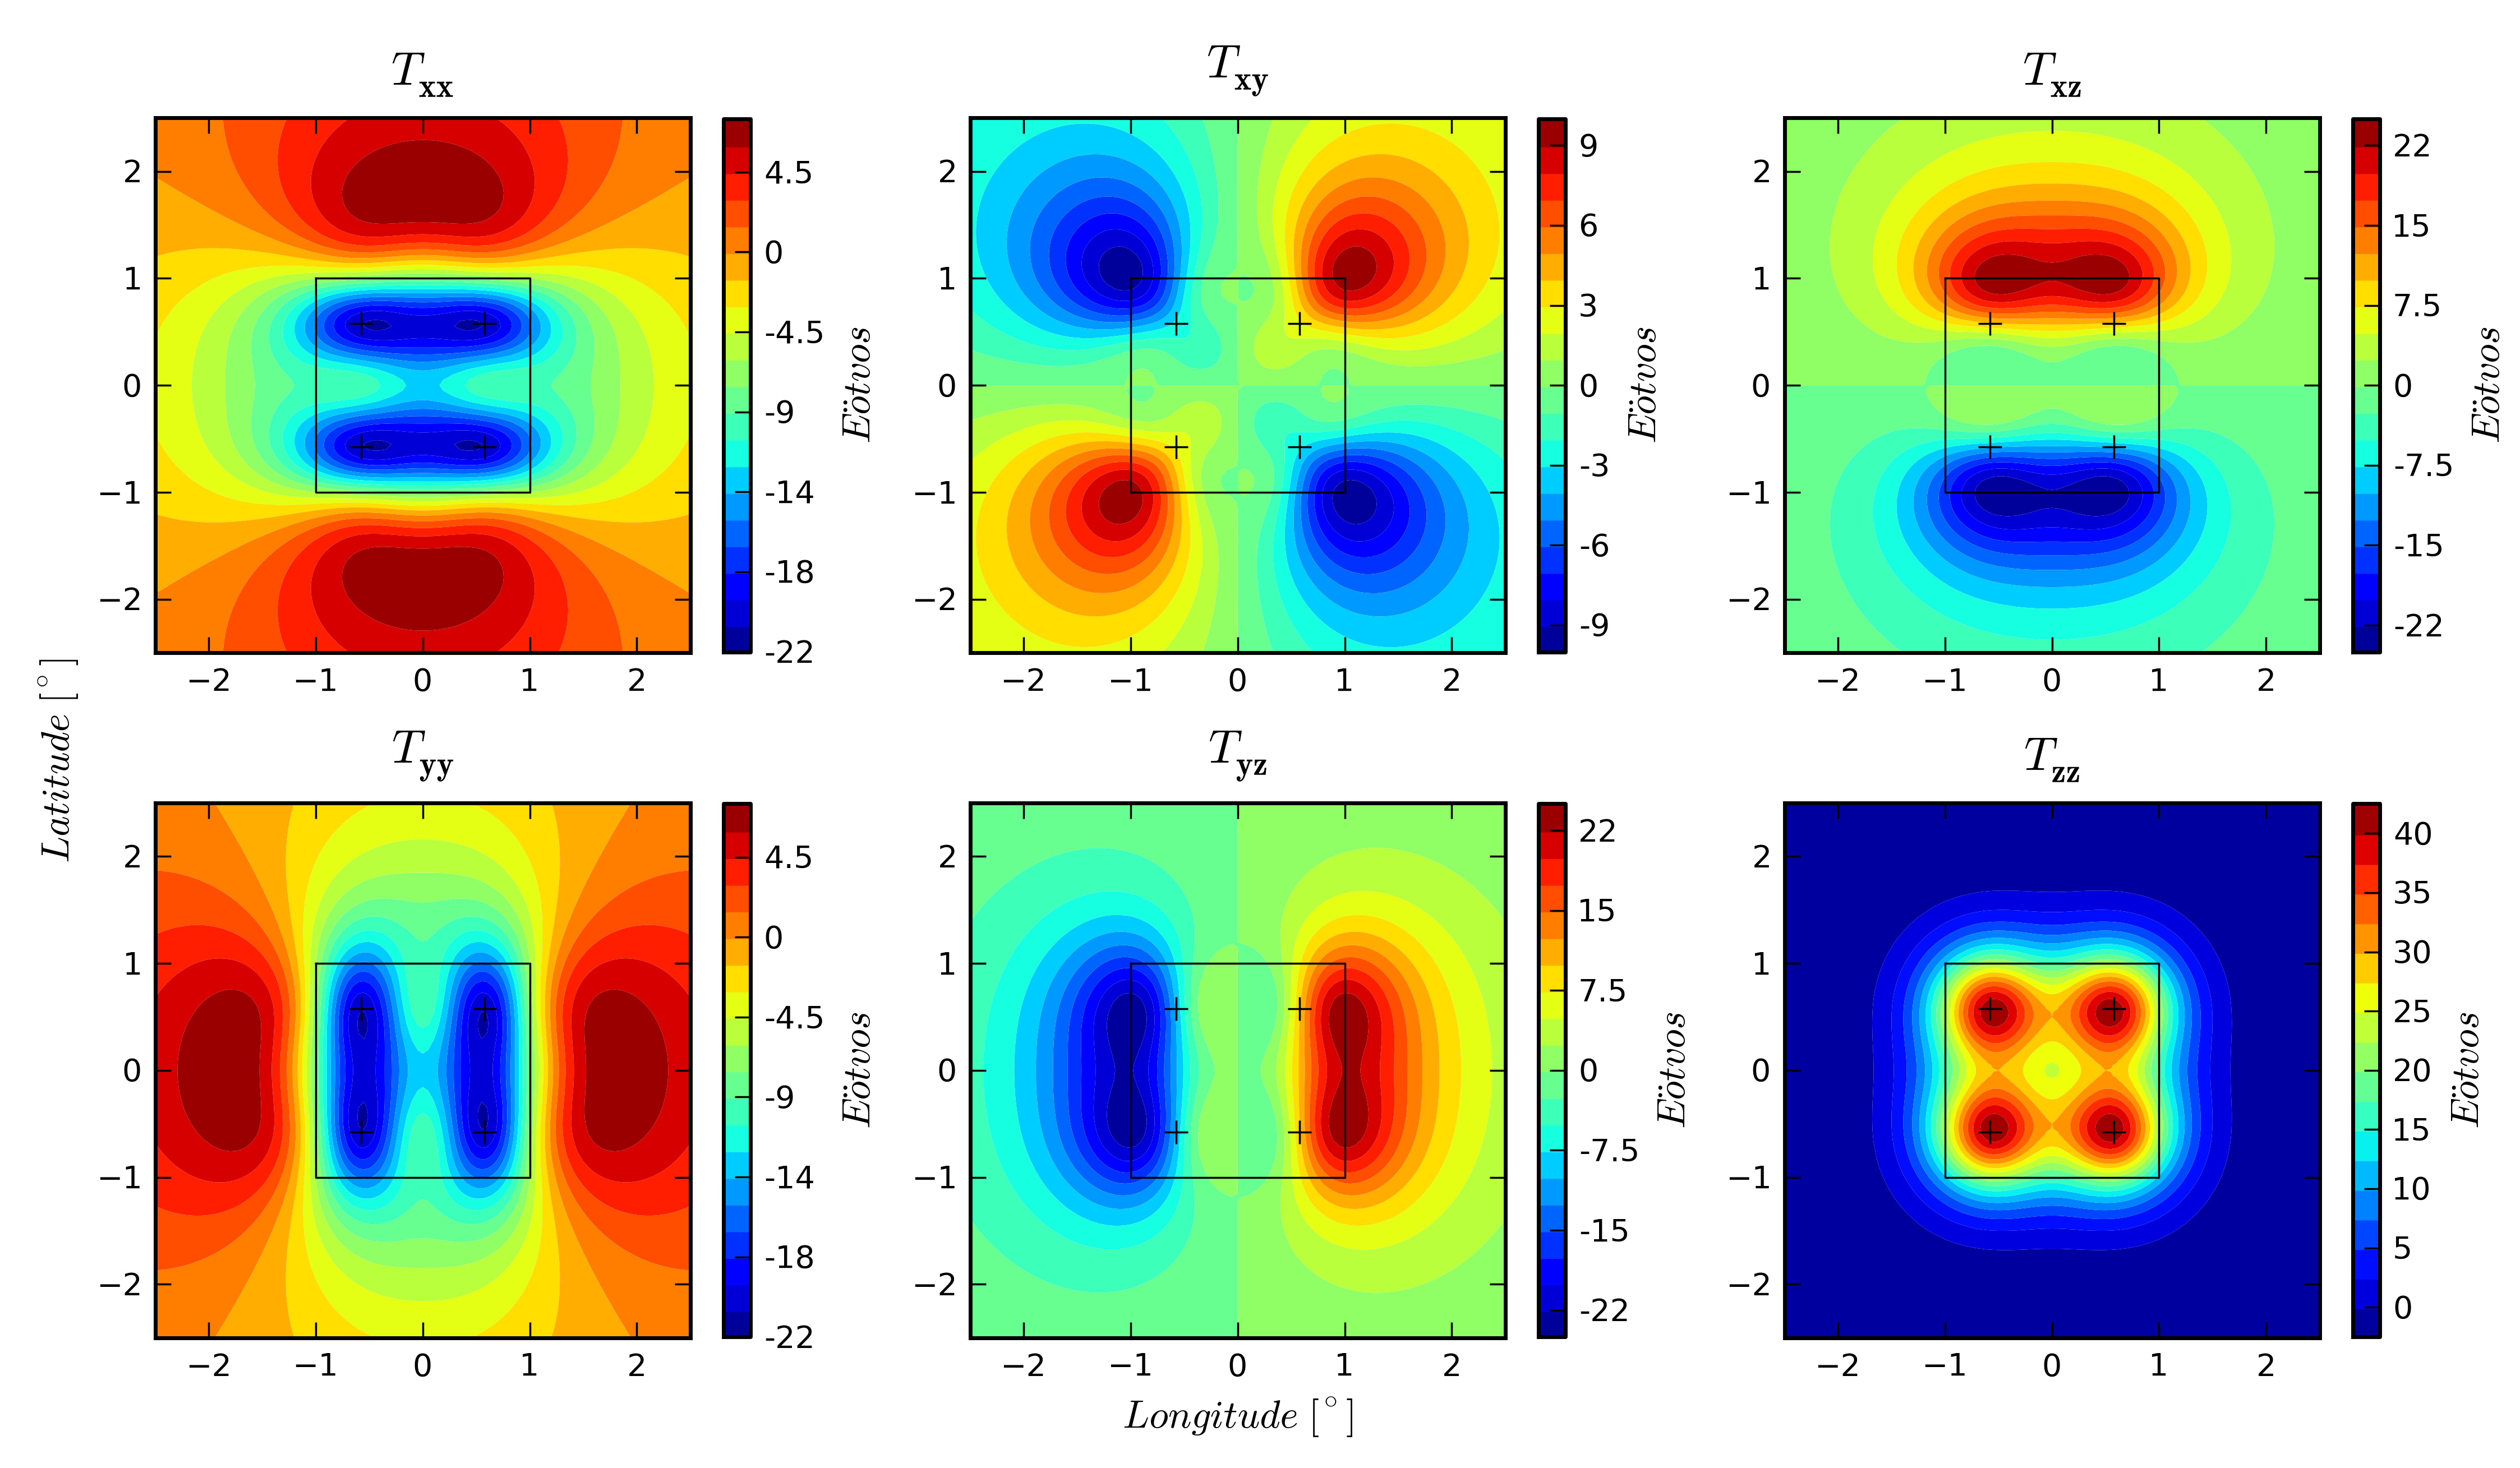
\includegraphics[scale=0.67]{../images/ggtT2x2at100-o2.png}
  \caption{\small TGG causado por um tesser�ide de
    $2^\circ \times 2^\circ \times 10\ km$, com densidade $2\ 800\ kg\ m^{-3}$,
    calculado a $100\ km$ de altitude. Quando a dist�ncia entre os n�s � maior
    que a dist�ncia ao ponto de observa��o, o TGG calculado aparenta ser causado
    por massas pontuais localizadas nos n�s, como pode ser observado claramente
    na componente $T_{zz}$.}
  \label{tgg-ku-100}
\end{figure}

\begin{figure}[!htb]
  \centering
    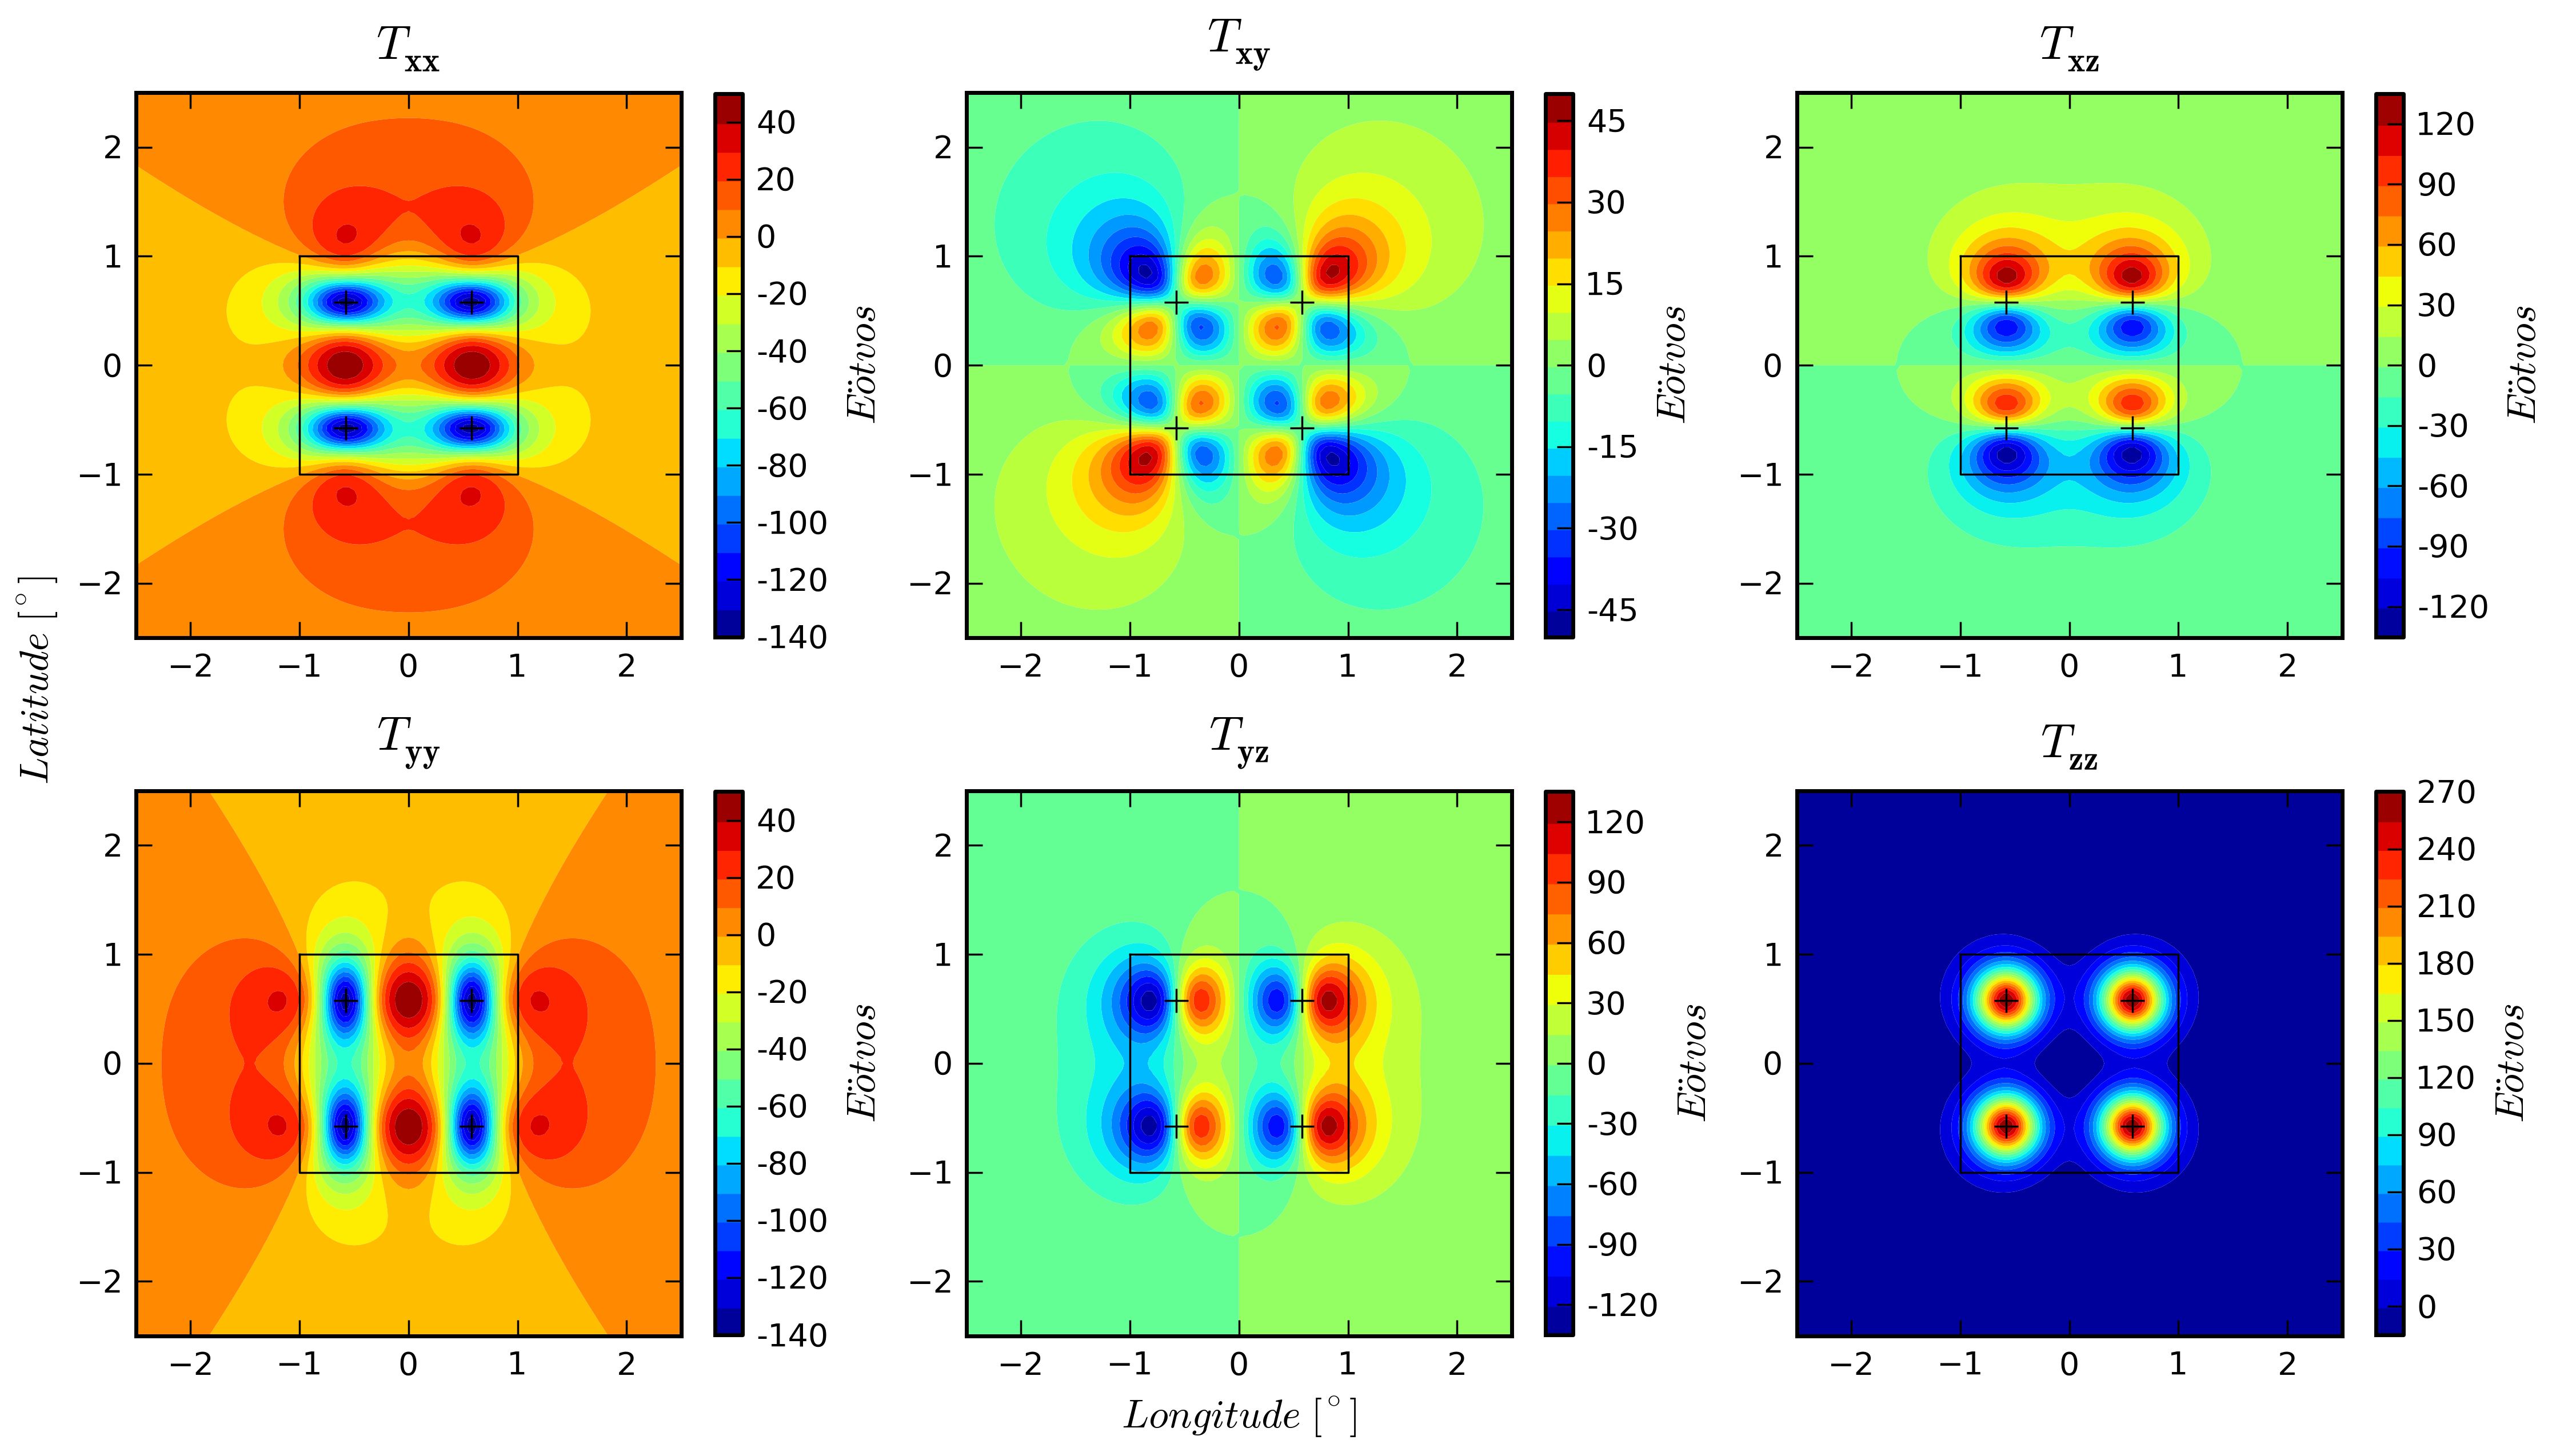
\includegraphics[scale=0.67]{../images/ggtT2x2at50-o2.png}
  \caption{\small TGG causado por um tesser�ide de
    $2^\circ \times 2^\circ \times 10\ km$, com densidade $2\ 800\ kg\ m^{-3}$,
    calculado a $50\ km$ de altitude. Neste caso � poss�vel notar que todas as
    componentes aparentam ser causadas por massas pontuais localizadas nos n�s.}
  \label{tgg-ku-50-o2}
\end{figure}

\begin{figure}[!htb]
  \centering
    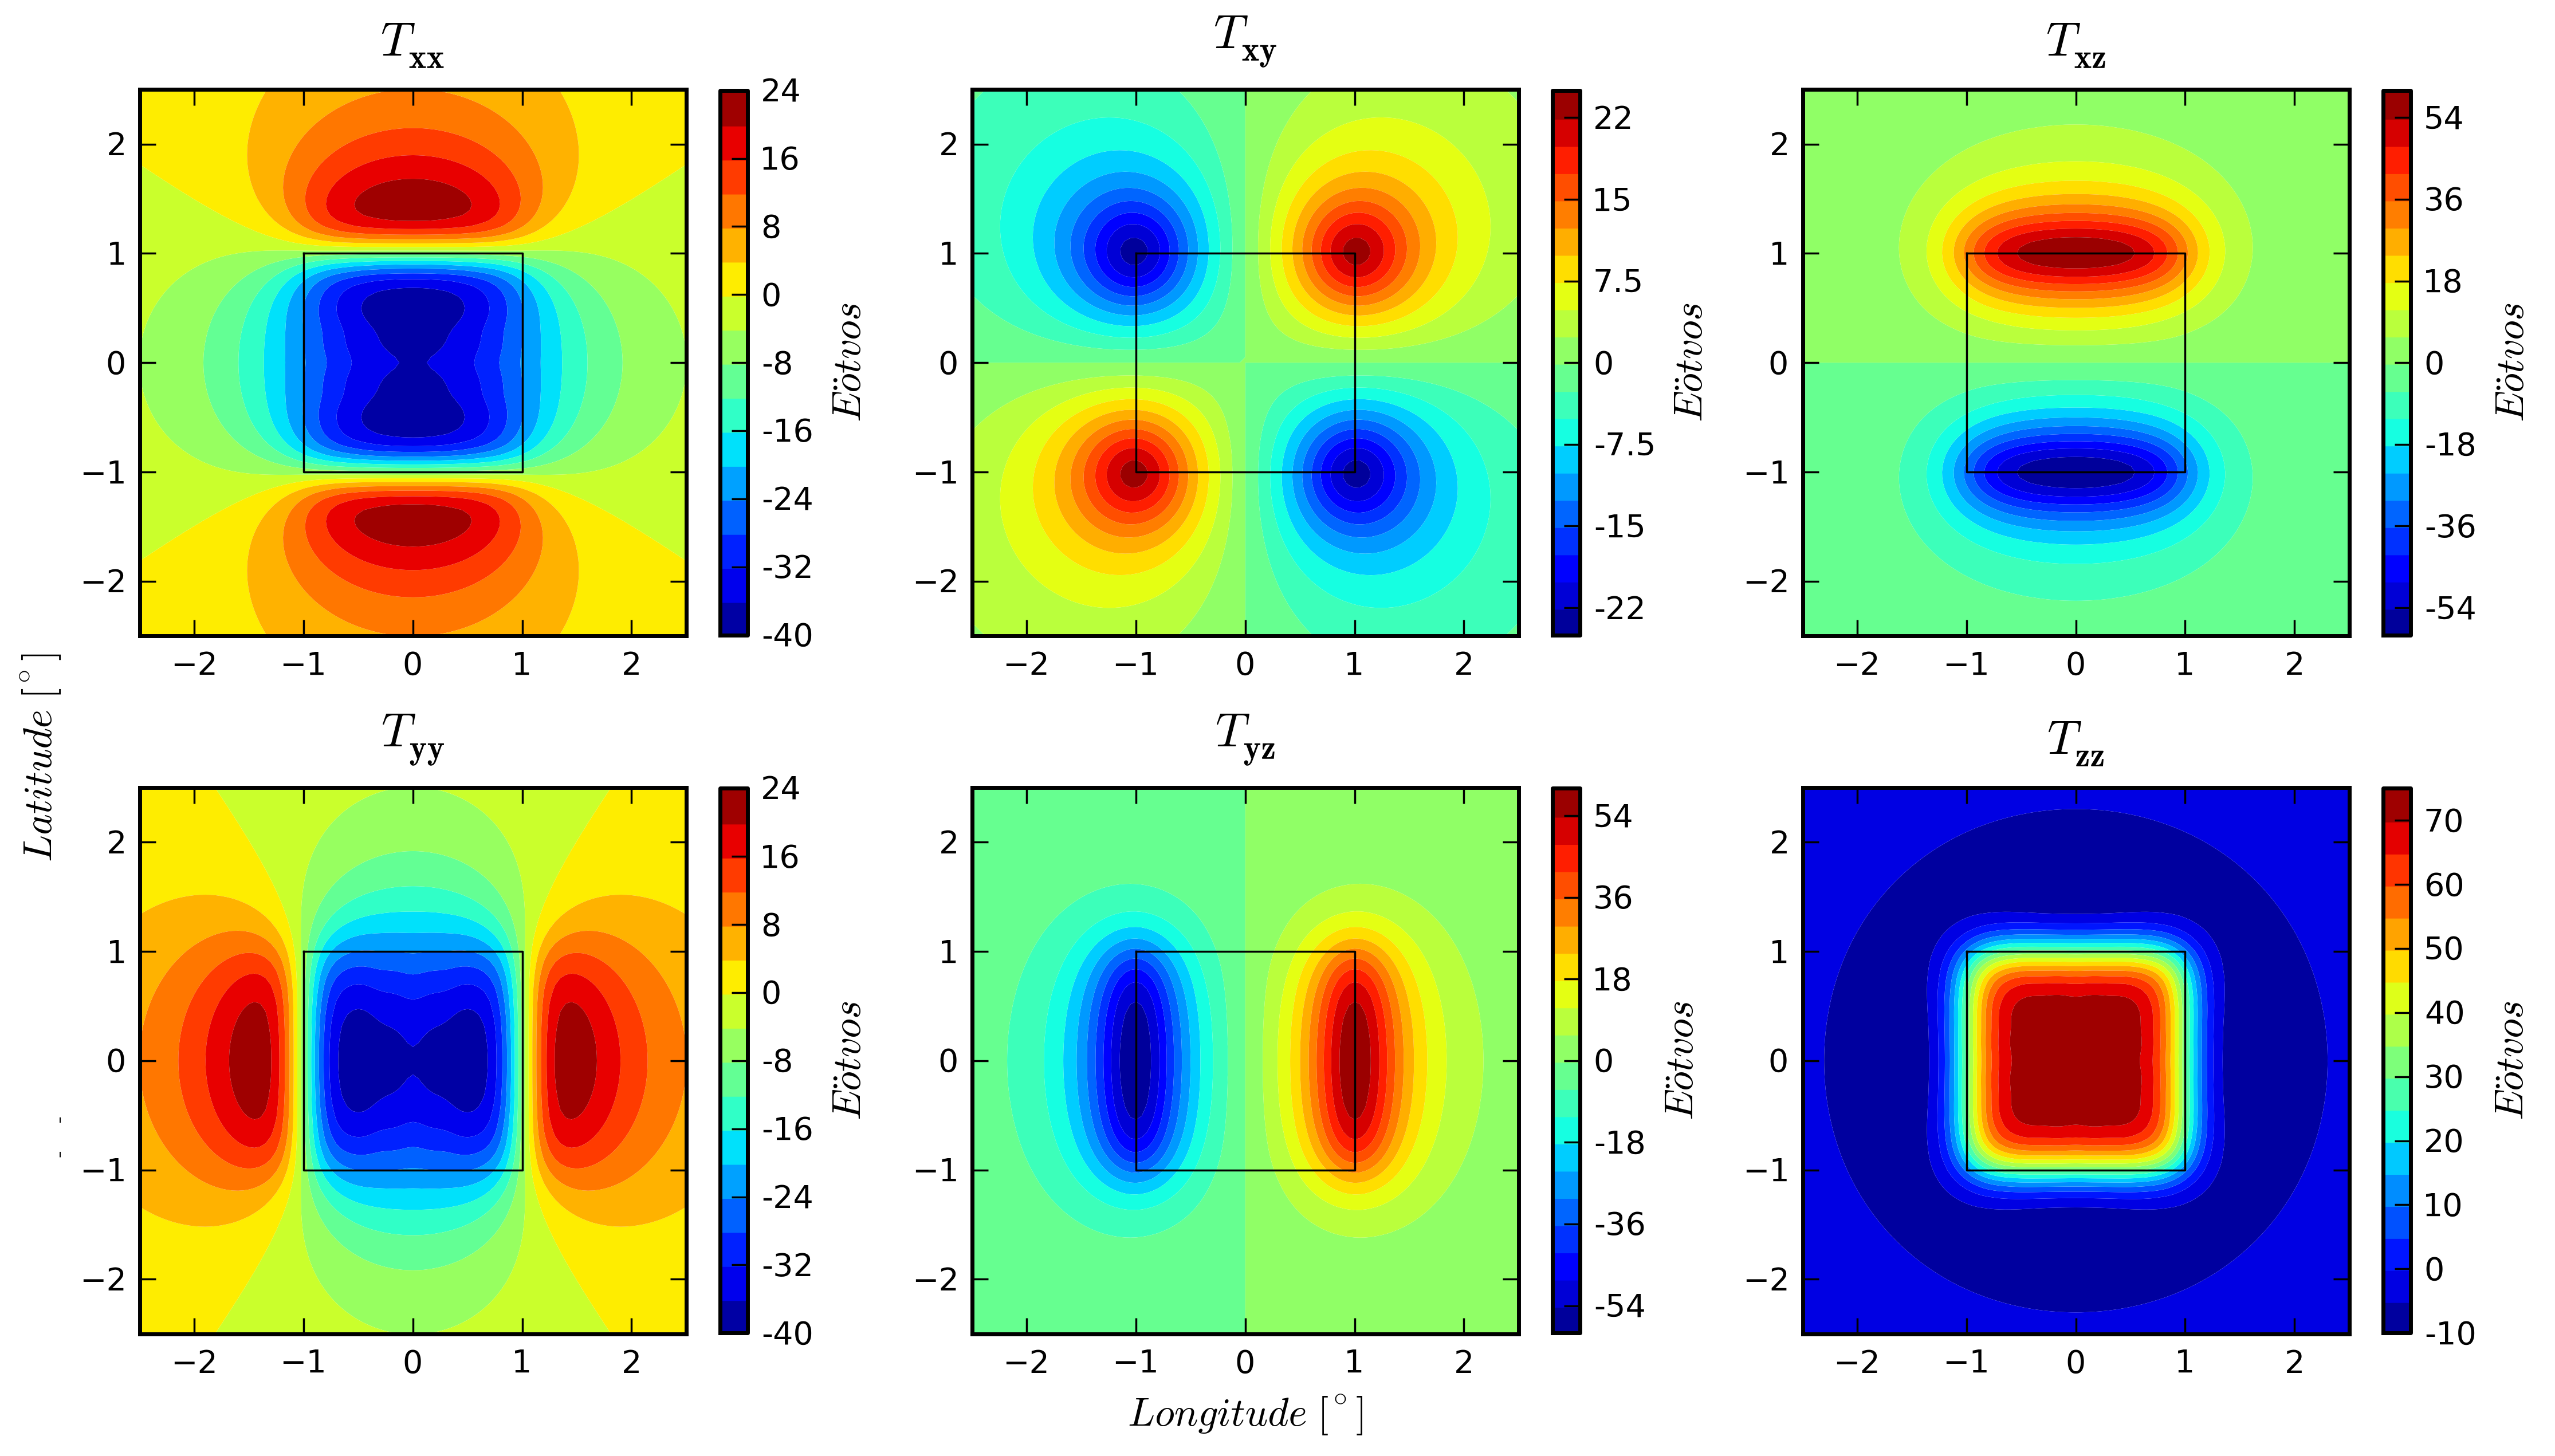
\includegraphics[scale=0.67]{../images/ggtT2x2at50-o10.png}
  \caption{\small TGG causado por um tesser�ide de
    $2^\circ \times 2^\circ \times 10\ km$, com densidade $2\ 800\ kg\ m^{-3}$,
    calculado a $50\ km$ de altitude.  A ordem utilizada foi
    $N_\varphi = N_\lambda = 10$ e dist�ncia m�xima entre dois n�s adjacentes �
    de aproximadamente $33\ km$. Como a dist�ncia entre os n�s � menor que a
    dist�ncia ao ponto de observa��o, o TGG calculado n�o aparenta ser devido a
    massas pontuais localizadas nos n�s e sim a um corpo volum�trico
    (tesser�ide).}
  \label{tgg-ku-50-o10}
\end{figure}

\begin{figure}[!htb]
  \centering
    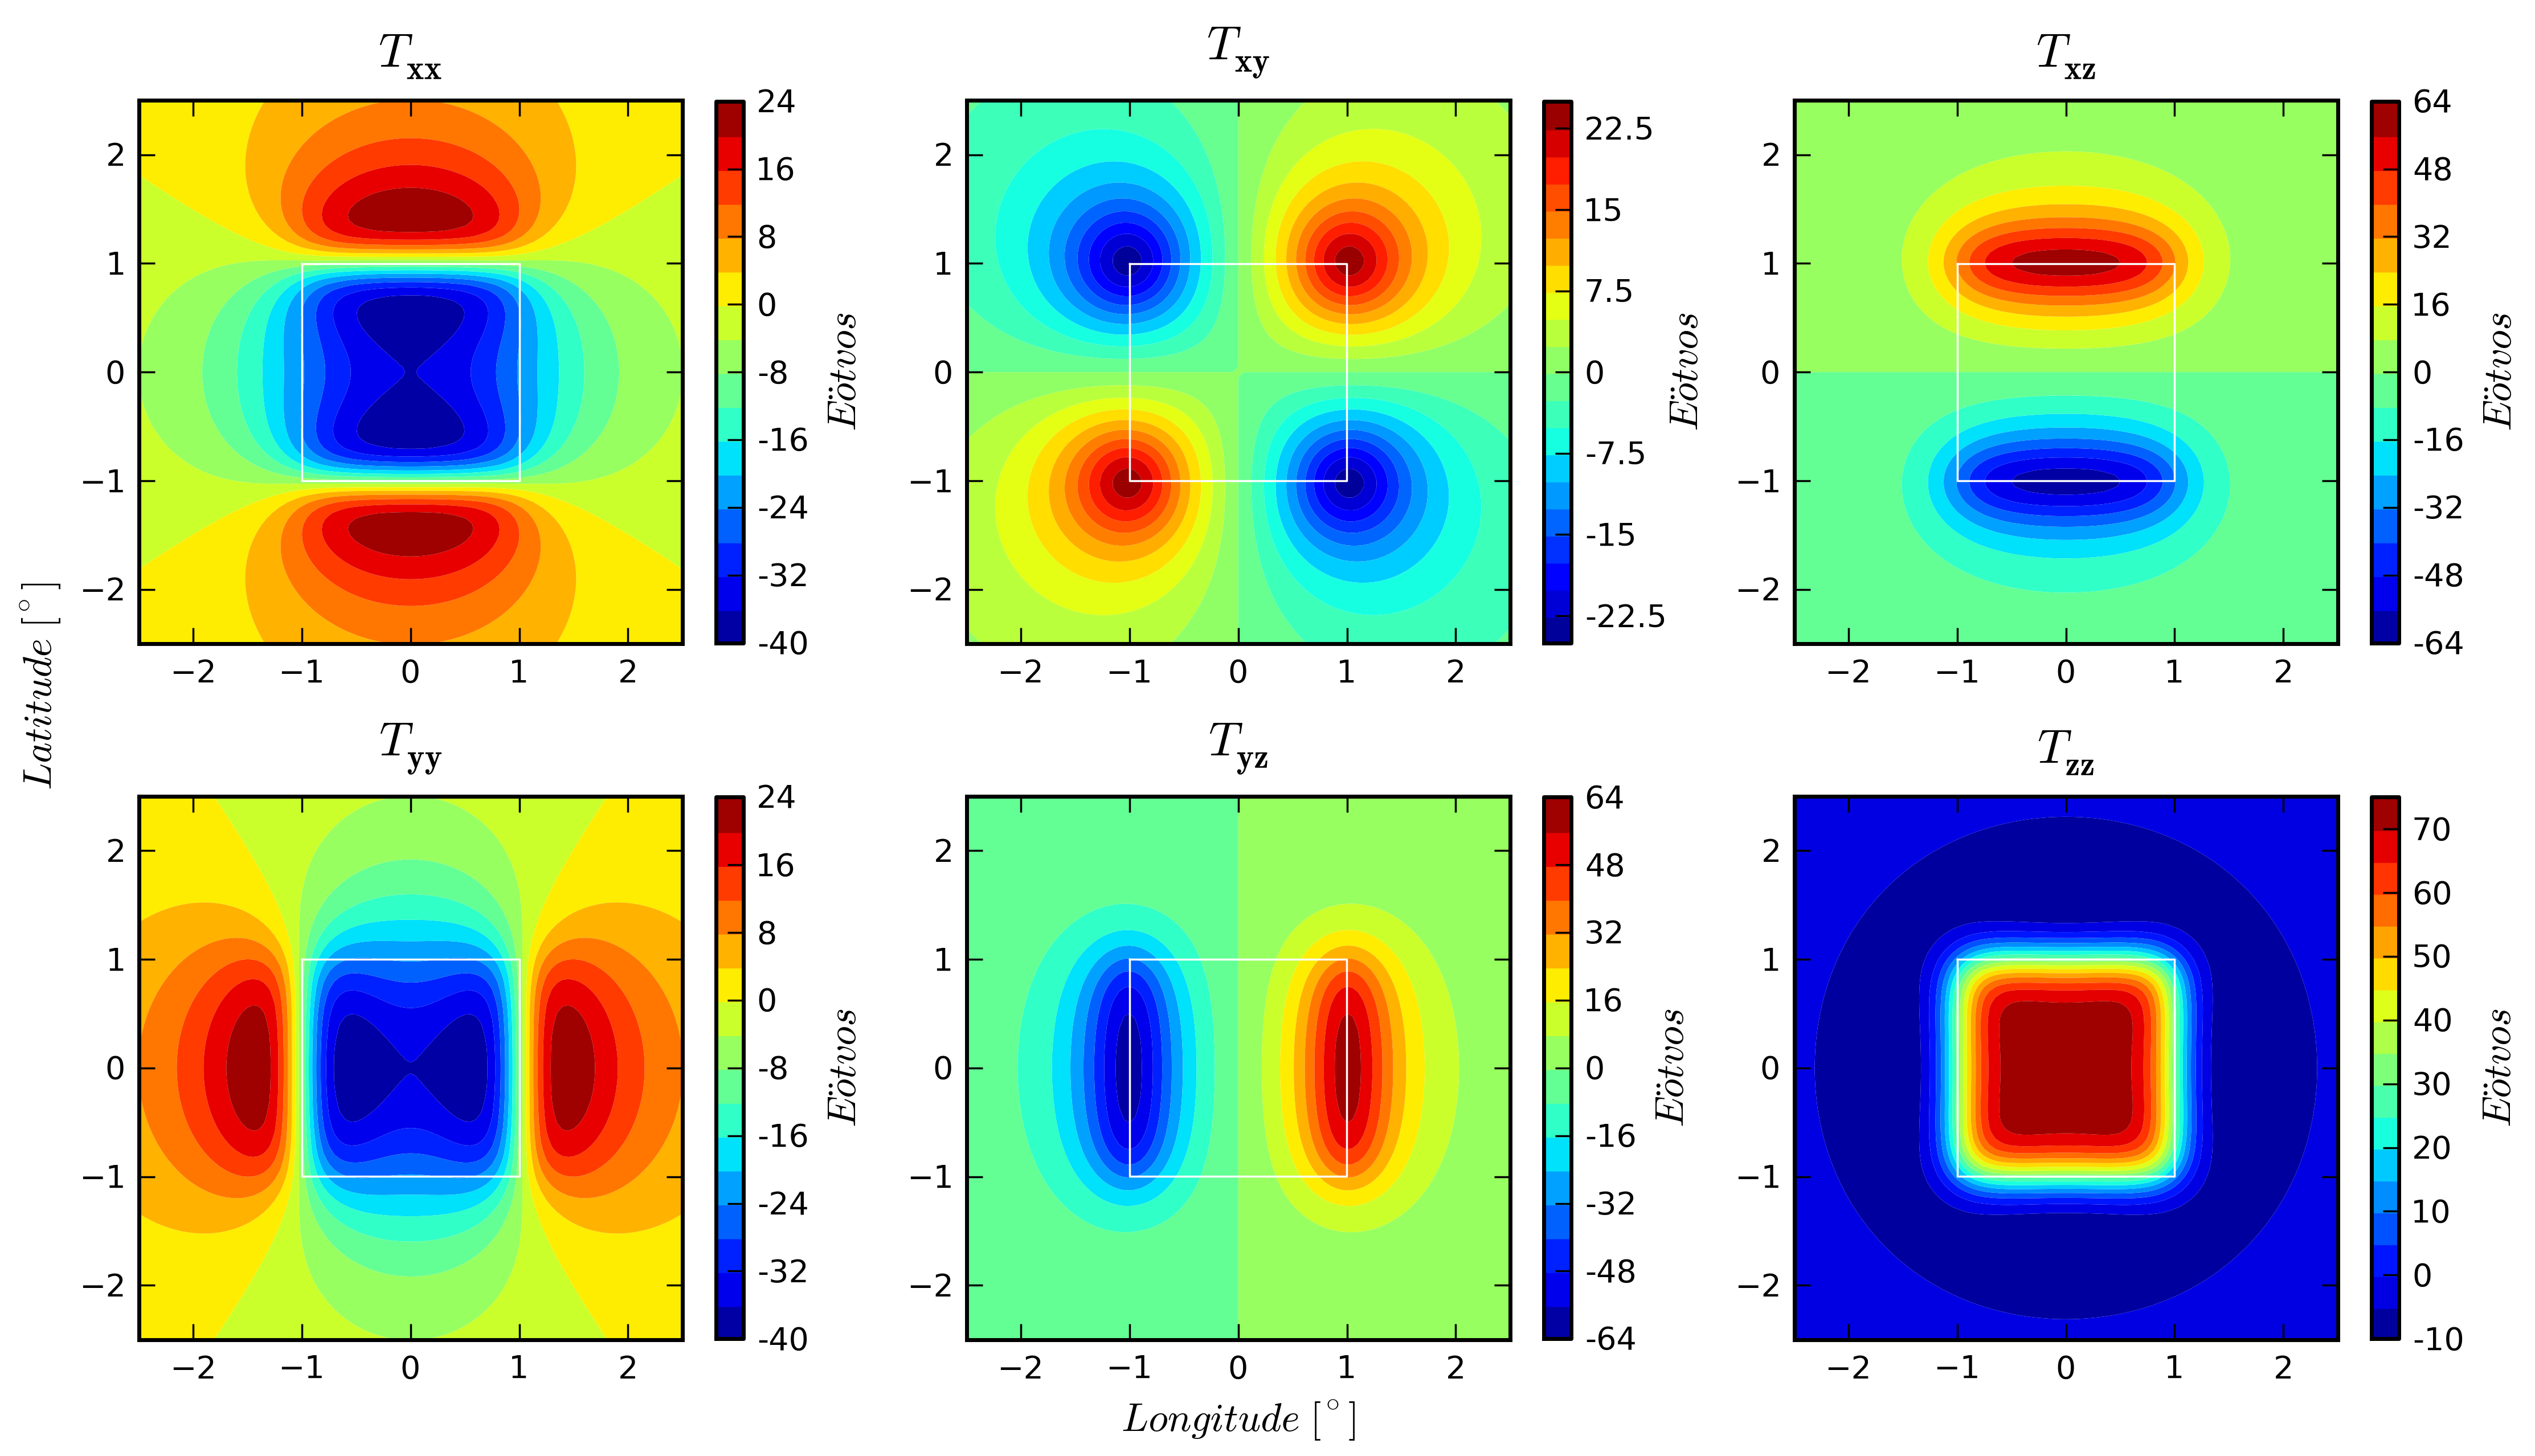
\includegraphics[scale=0.67]{../images/ggtP2x2at50.png}
  \caption{\small TGG causado por um prisma retangular que aproxima o tesser�ide de
    $2^\circ \times 2^\circ \times 10\ km$, com densidade $2\ 800\ kg\ m^{-3}$,
    calculado a $50\ km$ de altitude. As bordas do prisma est�o marcadas em
    branco.}
  \label{tgg-ku-50-prisma}
\end{figure}


\begin{figure}[!htb]
  \centering
    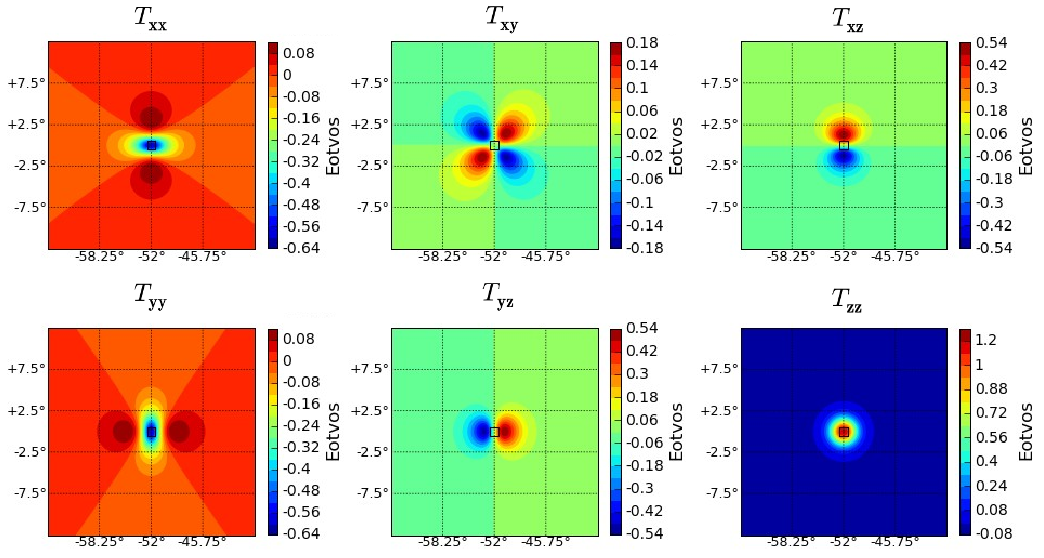
\includegraphics[scale=0.4]{../images/tess-plano-1.png}
  \caption{\small TGG causado por um tesser�ide de
    $1^\circ \times 1^\circ \times 10\ km$, com densidade $2\ 800\ kg\ m^{-3}$,
    e $N_\varphi = N_\lambda = 2$ calculado a $250\ km$ de altitude.}
  \label{tgg-tess1x1}
\end{figure}

\begin{figure}[!htb]
  \centering
    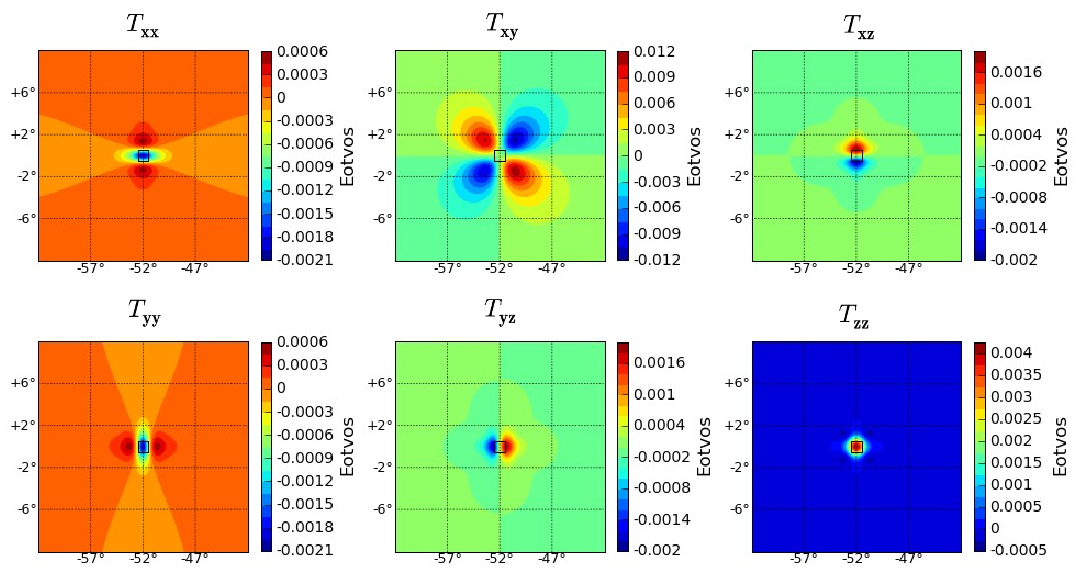
\includegraphics[scale=0.4]{../images/dif-plano-1.png}
  \caption{\small Diferen�a entre o TGG causado pelo tesser�ide da Figura
    \ref{tgg-tess1x1} e o causado por um prisma de mesma massa utilizando uma
    aproxima��o plana para a Terra esf�rica. Nesta aproxima��o os sistemas
    locais dos pontos de observa��o possuem a mesma orienta��o do sistema local
    do corpo plano e $1^\circ$ de latitude ou longitude equivale a $111,11\ km$.
    As diferen�as chegam a aproximadamente 7\% na componente $T_{xy}$, por�m
    n�o passam de 0.5\% na componente $T_{zz}$.}
  \label{tgg-dif1x1}
\end{figure}

\begin{figure}[!htb]
  \centering
    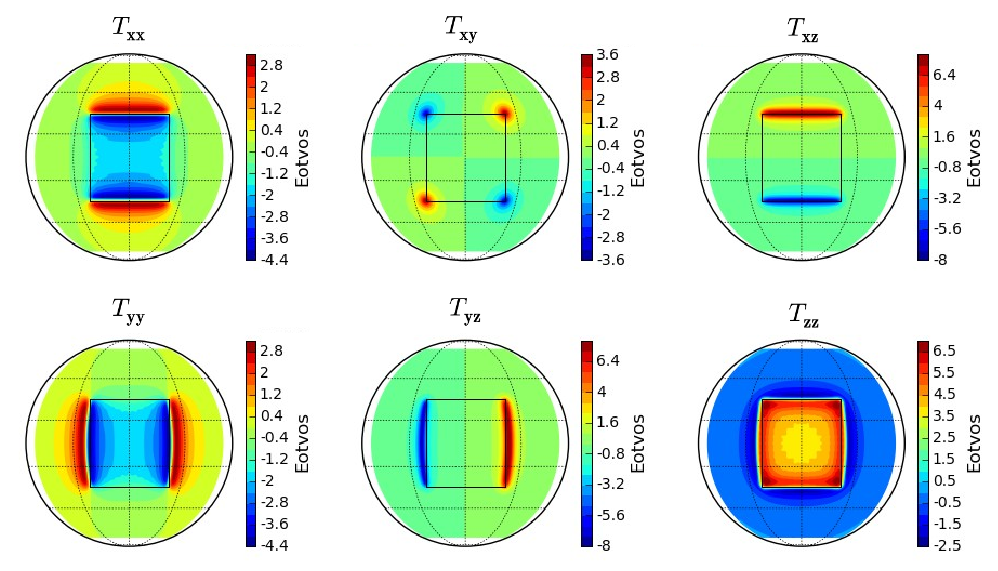
\includegraphics[scale=0.4]{../images/tess-plano-50.png}
  \caption{\small TGG causado por um tesser�ide de
    $50^\circ \times 50^\circ \times 10\ km$, com densidade $2\ 800\ kg\ m^{-3}$
    e calculado a $250\ km$ de altitude.}
  \label{tgg-tess50x50}
\end{figure}

\begin{figure}[!htb]
  \centering
    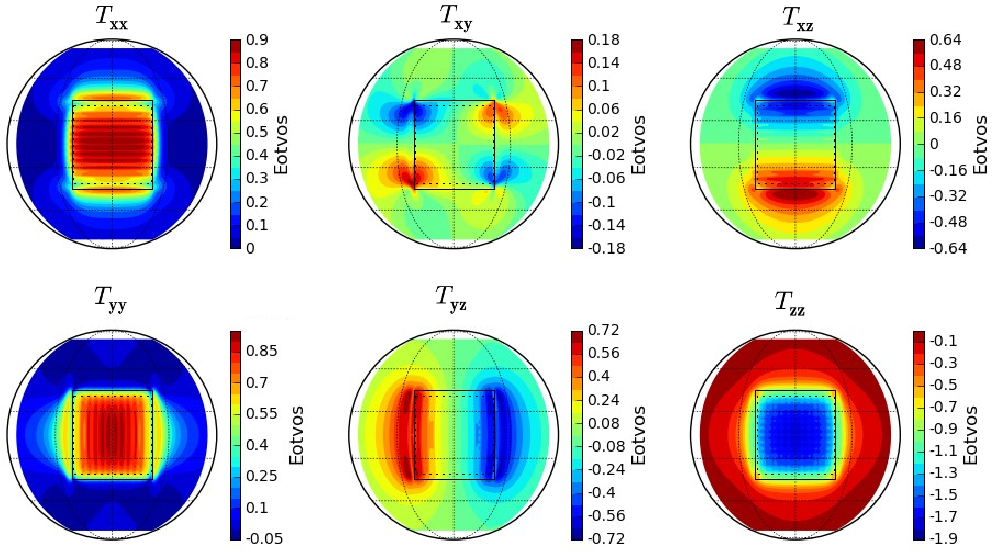
\includegraphics[scale=0.4]{../images/dif-plano-50.png}
  \caption{\small Diferen�a entre o TGG causado pelo tesser�ide da Figura
    \ref{tgg-tess50x50} e o causado por um prisma de mesma massa utilizando uma
    aproxima��o plana para a Terra esf�rica. Neste caso, as diferen�as chegam a
    aproximadamente 30\% na componente $T_{zz}$ e aproximadamente 5\% na
    componente $T_{xy}$.}
  \label{tgg-dif50x50}
\end{figure}


\begin{figure}[!htb]
  \centering
    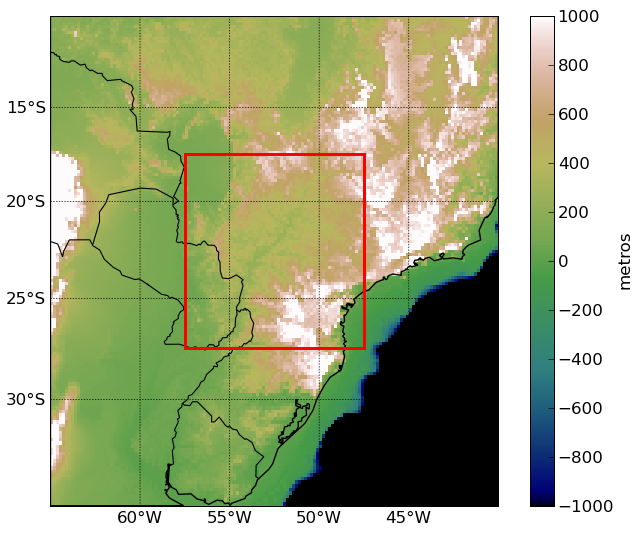
\includegraphics[scale=0.5]{../images/topografia-10min-marca-grid.png}
  \caption{\small Modelo topogr�fico digital ETOPO1 utilizado para gerar o modelo de
    tesser�ides. O espa�amento da grade � de $10'\times10'$. Em vermelho est�
    marcada a �rea na qual o TGG foi calculado. }
  \label{topografia}
\end{figure}

\begin{figure}[!htb]
  \centering
    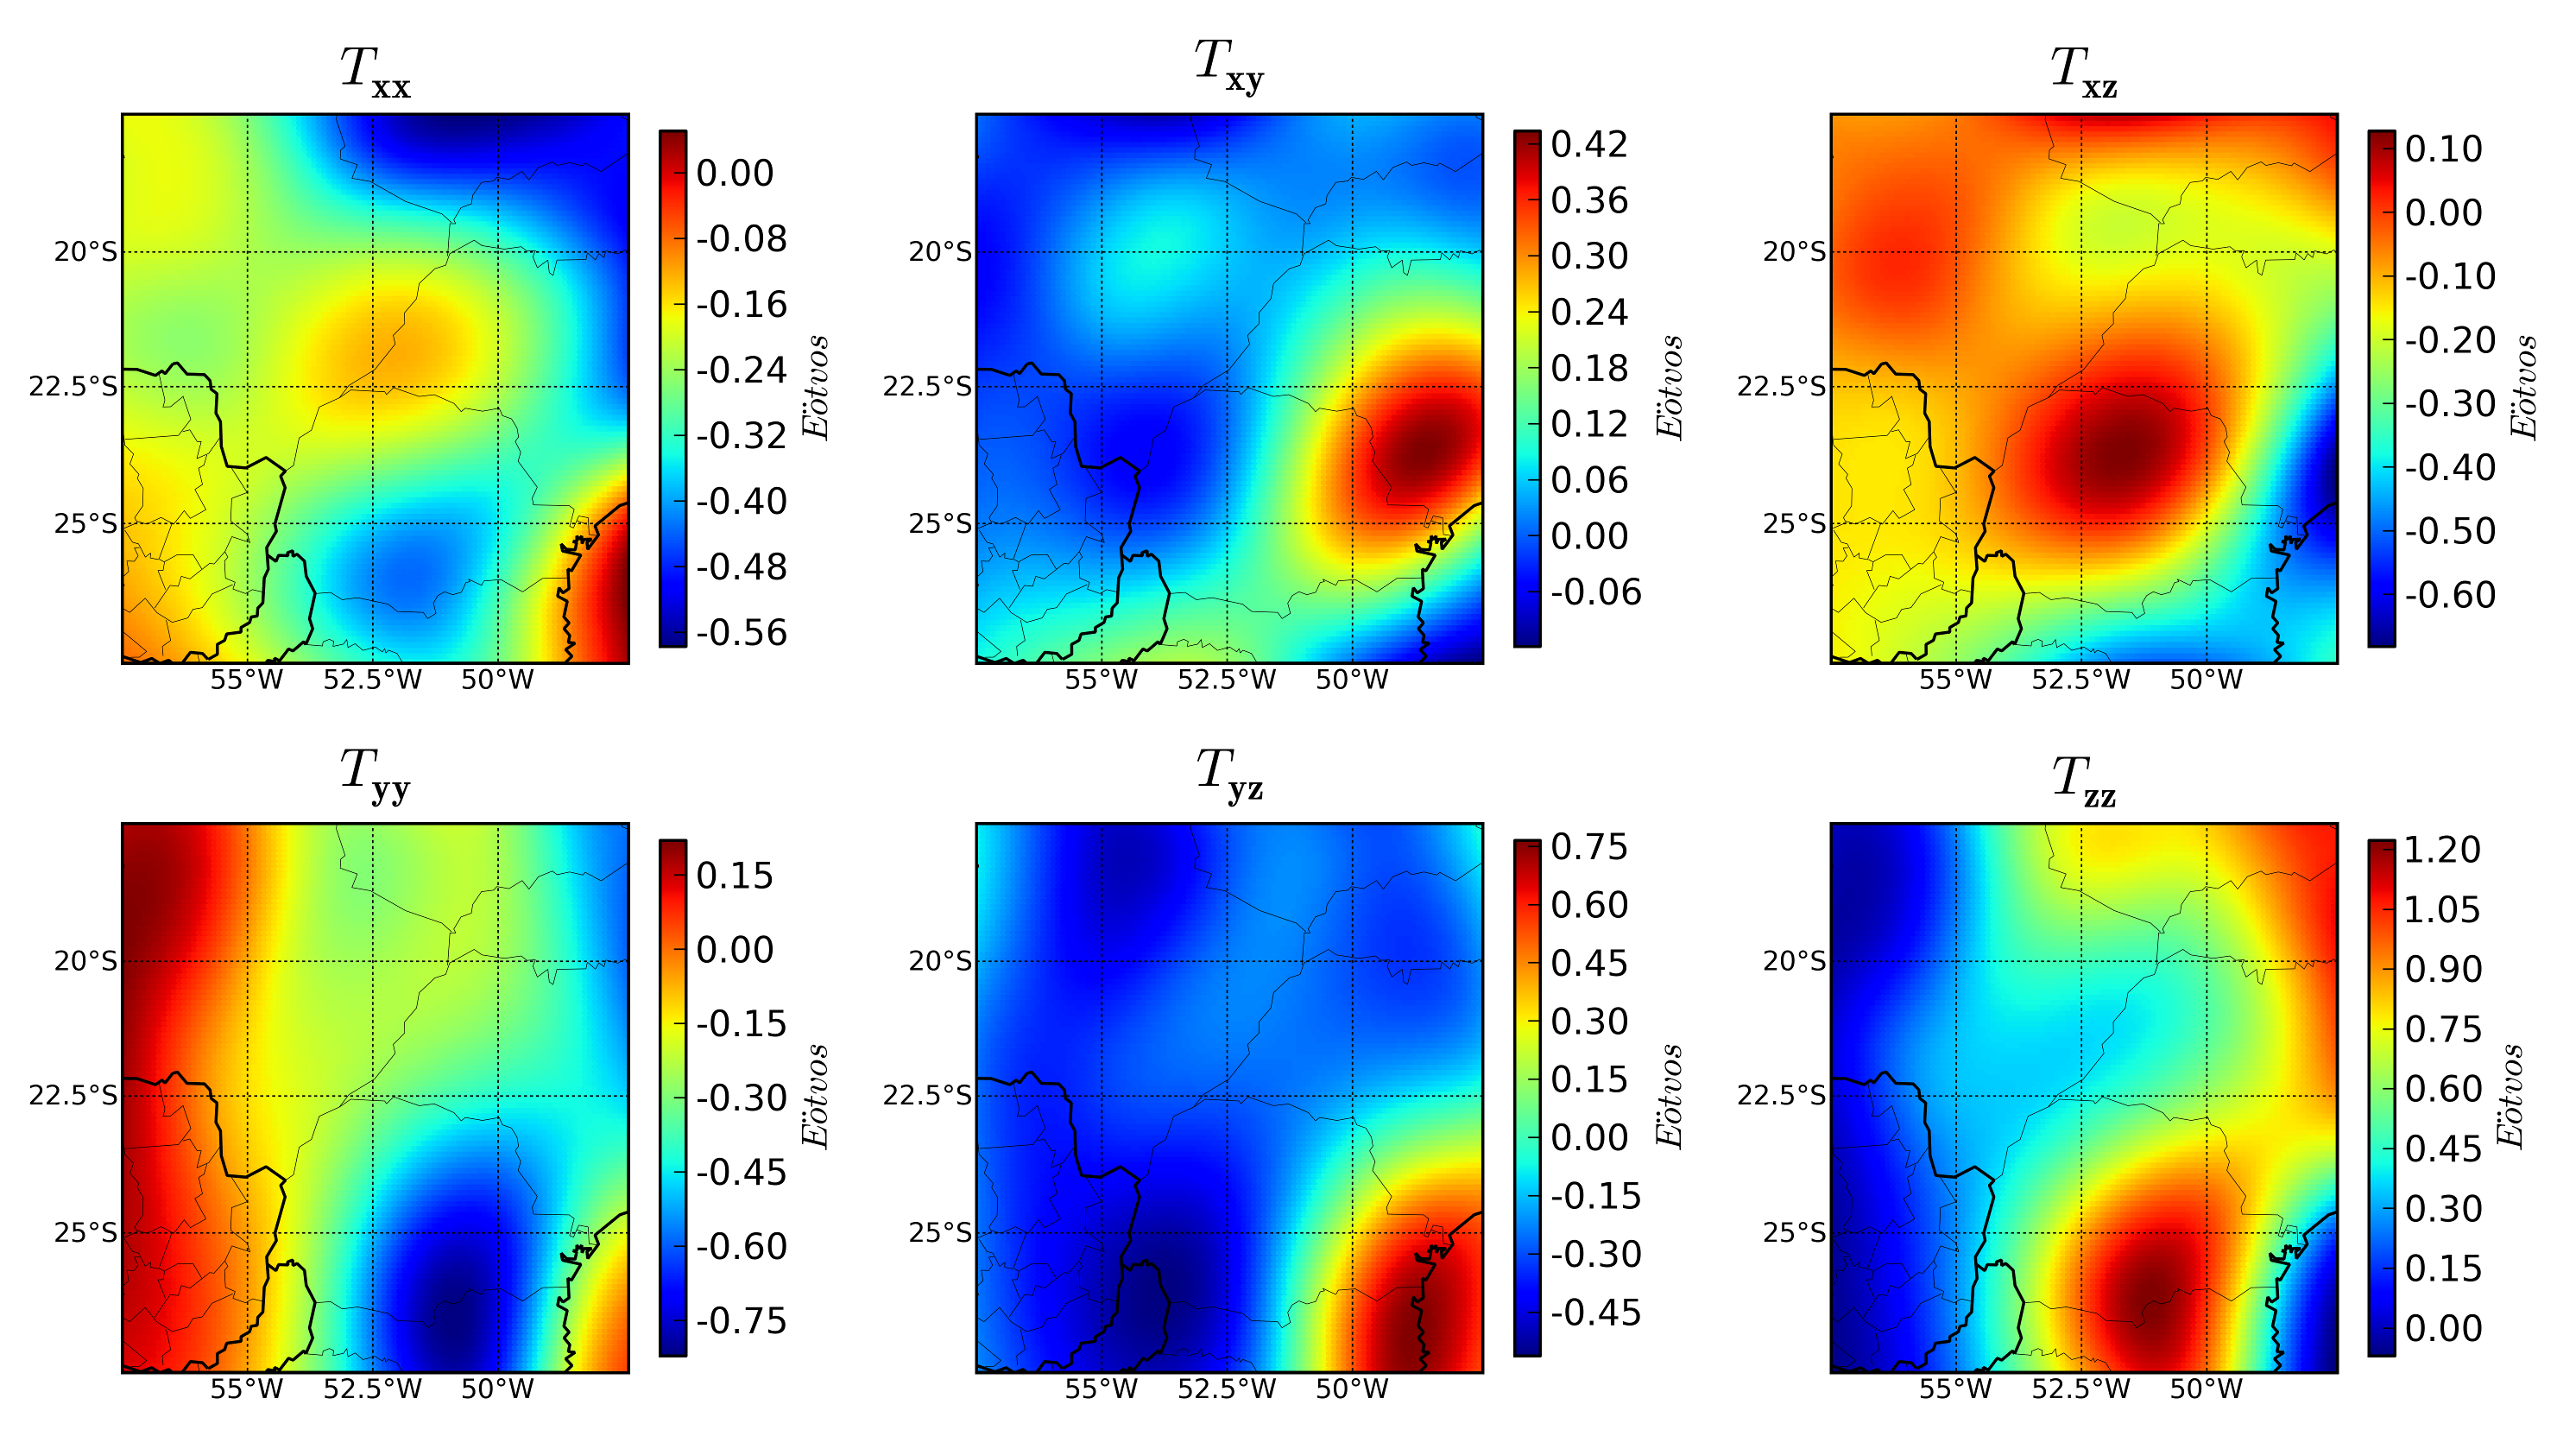
\includegraphics[scale=1]{../images/topoeffect-10m-tgg-tmp.png}
  \caption{\small Efeito da topografia no TGG a $250\ km$ de altitude na regi�o da
    Bacia do Paran�. Foi utilizada densidade de $2\ 670\ kg\ m^{-3}$ e
    $N_\varphi = N_\lambda = 2$. Este � um efeito significativo em todas as
    componentes e deve ser levado em conta durante a modelagem de dados de TGG.}
  \label{tgg-topografia}
\end{figure}

  % Concluso
  \chapter{Conclus�o}

O programa computacional implementado na linguagem Python � confi�vel pois
possui ``unit tests'' e ``testes de integra��o'' que verificam automaticamente
a funcionalidade de cada parte do programa e seu funcionamento como um todo.
As fun��es e classes implementadas poder�o ser facilmente reutilizadas em outros
programas devido � modularidade inerente na linguagem Python.
Al�m disso, as singularidades presentes na metodologia de Wild-Pfeiffer (2008)
foram efetivamente contornadas utilizando a integra��o num�rica 3D nos pontos
onde ocorrem.
\\
\indent Foi observado que o TGG de um tesser�ide calculado utilizando a QGL
apresenta o mesmo artefato num�rico observado por Ku (1977).
Por isso, a ordem da QGL deve ser escolhida de tal forma que a dist�ncia entre
os n�s seja menor que a dist�ncia at� o ponto de observa��o.
Isso significa que, a altitude de 250 km, o TGG de um tesser�ide com face de
at� $2^\circ \times 2^\circ$ pode ser calculado utilizando ordem dois.
\\
\indent No caso dos an�is de massa com ponto de observa��o em
$\varphi = 90^\circ$, o programa desenvolvido apresentou resultados com precis�o
semelhante aos apresentados em Wild-Pfeiffer (2008).
As componentes $T_{xy}$ e $T_{yy}$ se mostraram inst�veis, o que era
esperado pois existem singularidades nas equa��es para este ponto de observa��o.
Este � um caso limite que deve ser evitado na pr�tica para garantir resultados
precisos.
\\
\indent A compara��o entre a modelagem com tesser�ides e uma aproxima��o plana
para a Terra esf�rica mostrou diferen�as de at� 30\% na componente $T_{zz}$
para um modelo de $50^\circ \times 50^\circ \times 10\ km$.
Esta � um diferen�a consider�vel que deve ser levada em conta na modelagem de
estruturas extensas.
\\
\indent O TGG devido � topografia da regi�o da bacia do Parana possui a mesma
ordem de grandeza nas amplitudes das componentes do TGG de um tesser�ide de
$1^\circ \times 1^\circ \times 10\ km$.
Isso mostra que o efeito topogr�fico deve ser removido dos dados que ser�o
observados na miss�o GOCE a fim de isolar o efeito dos corpos an�malos em
subsuperf�cie.

  
  
  



  % Referncias
  \bibliographystyle{plainnat}
\begin{thebibliography}{20}
\addcontentsline{toc}{chapter}{Refer�ncias}
\begin{small}

  \bibitem[Amante e Eakins (2009)]{amante&eakins2009} AMANTE, C.; EAKINS, B.W. ETOPO1 1 Arc-Minute Global Relief Model: Procedures, Data Sources and Analysis. \textbf{NOAA Technical Memorandum NESDIS NGDC-24}, p. 19, 2009.

  \bibitem[Asgharzadeh \textit{et al.} (2007)]{asgharzadeh_etal2007} ASGHARZADEH, M.F.; VON FRESE, R.R.B.; KIM, H.R.; LEFTWICH, T.E.; KIM, J.W. Spherical prism gravity ef\mbox{}fects by Gauss-Legendre quadrature integration. \textbf{Geophysics Journal International}, v. 169, p. 1-11, 2007.

  \bibitem[Barrera-Figueroa \textit{et al.} (2006)]{barrera-figueroa_etal2006} BARRERA-FIGUEROA, V.; SOSA-PEDROZA, J.; L�PEZ-BONILLA, J. Multiple root finder algorithm for Legendre and Chebyshev polynomials via Newton's method. \textbf{Annales Mathematicae et Informaticae}, v. 33, p. 3 - 13, 2006.
 
  \bibitem[Heck e Seitz (2007)]{heck&seitz2007}HECK, B.; SEITZ, K. A comparison of the tesseroid, prism and point-mass approaches for mass reductions in gravity field modelling. \textbf{Journal of Geodesy}, v. 81, p. 121 - 136, 2007.

  \bibitem[Heiskanen and Moritz (1967)]{h&m1967} HEISKANEN, W.A.; MORITZ, H. \textbf{Physical Geodesy}. W. H. Freeman and Company, San Francisco, 1967.

  \bibitem[Hildebrand (1987)]{hildebrand1987} HILDEBRAND. F.B.  \textbf{Introduction to numerical analysis}. Courier Dover Publications, 2. ed., 1987.

  \bibitem[Ku (1977)]{ku1977} KU, C.C. A direct computation of gravity and magnetic anomalies caused by 2- and 3-dimensional bodies of arbitrary shape and arbitrary magnetic polarization by equivalent-point methot and a simplified cubic spline. \textbf{Geophysics}, v. 42, p. 610 - 622, 1977.

%   \bibitem[Makhloof e Ilk (2008)]{makhloof&ilk2008} MAKHLOOF, A.A.; ILK, K. Effects of topographic-isostatic masses on gravitational functionals at the Earth's surface and at airborne and satellite altitudes. \textbf{Journal of Geodesy}, v. 82, p. 93 - 111, 2008.

%   \bibitem[Nagy (1966)]{nagy1966} NAGY, D. The gravitational attraction of a right rectangular prism. \textbf{Geophysics}, v. 31, p. 362 - 371, 1966.


  \bibitem[Nagy (2000)]{nagy2000} NAGY, D.; PAPP, G.; BENEDEK, J. The gravitational potential and its derivatives for the prism. \textbf{Journal of Geodesy}, v. 74, p. 552 - 560, 2000.


  \bibitem[Press \textit{et al.} (1992)]{numericalrecipes} PRESS, W.H.; FLANNERY, B.P.; TEUKOLSKY, S.A.; VETTERLING, W.T. \textbf{Numerical Recipes in C: The Art of Scientific Computing}. Cambridge University Press, 2. ed., 1992.

  \bibitem[Smith, Robertson e Milbert (2001)]{smith_etal2001} SMITH, D.A.; ROBERTSON, D.S.; MILBERT, D.G. Gravitational attraction of local crustal masses in spherical coordinates. \textbf{Journal of Geodesy}, v. 74, p. 783 - 795, 2001.

  \bibitem[Tscherning (1976)]{tscherning1976} TSCHERNING, C.C. Computation of the second-order derivatives of the normal potential based on the representation by a Legendre series. \textbf{Manuscripta Geodaetica}, v. 1, p. 71 - 92, 1976.

  \bibitem[Van�\v{c}ek e Krakiwsky (1986)]{vanicek1986} VAN�\v{C}EK, P.; KRAKIWSKY, E. \textbf{Geodesy: The Concepts}. Elsevier Science Publishers B.V., 2. ed., 1986.

  \bibitem[Wild-Pfeiffer (2008)]{wild-pfeiffer2008} WILD-PFEIFFER, F. A comparison of different mass elements for use in gravity gradiometry. \textbf{Journal of Geodesy}, v. 82 (10), p. 637 - 653, 2008.
\end{small}
\end{thebibliography}




\end{document}